\documentclass{article}
\usepackage{soul}
\usepackage{xcolor}  % 需要这个包来改变颜色
\sethlcolor{yellow}  % 设置highlight的颜色为红色
\usepackage{amsmath}
\usepackage{amssymb}
\usepackage{cancel}
\usepackage{graphicx}
\usepackage{tikz}


\title{MATH1064}
\author{Usyd Mingyuan Ba}
\date{\today}

\begin{document}

\maketitle

\section{Week1}
(i) \textbf{Definitions}
\begin{itemize}
\item Propositions : A proposition is a sentence that is true or false but \hl{not both}.

\item Variables and Compound Propositions : We use capital letters for compound propositions, which are made up from
proposition variables (e.g. p, q,r, ...) and the symbols with $\land , \lor , \neg$ and
unambiguous parentheses.

\item Logical equivalence : Two compound propositions P and Q are logically equivalent:\\
\hl{$P \equiv Q$}\\
if they have identical truth values for every possible combination of truth
values for their proposition variables.

\item Contradiction : A contradiction is a compound proposition which takes the value false \hl{for
all possible truth values (true/false in all combinations)} of its variables.\\
Examples: $p \land \neg p$ ,$(q \land p) \land \neg p$

\item Tautology : A tautology is a compound proposition which takes the value true \hl{for all
possible truth values (true/false in all combinations)} of its variables.\\
Examples: $p \lor \neg p$

================================================================================================================
\newpage
================================================================================================================


\item The conditional : Let p and q be proposition variables; the conditional from p to q, p $\rightarrow$ q,
is defined by the following truth table:

\begin{tabular}{ccc}
  p & q & p $\rightarrow$ q \\
  T & T & T \\
  T & F & F \\
  F & T & T \\
  F & F & T \\
\end{tabular}

\hl{p is the hypothesis and q is the conclusion.}

\hl{Different ways of saying p $\rightarrow$ q:}\\
1 p implies q\\
2 if p, then q\\
3 q if p\\
4 p only if q\\
5 p is sucient for q\\
6 q is necessary for p\\

p $\rightarrow$ q is false if and only if it describes a counterexample;
that is, the hypothesis is true but the conclusion is false.\\

\hl{$p \rightarrow q \equiv \neg p \lor q$}

\item Converse : The converse of $p \rightarrow q$ is $q \rightarrow p.$ 

\item Inverse : The inverse of $p \rightarrow q$ is $ \neg p \rightarrow \neg q.$

\item The biconditional :  Let p and q be proposition variables; the biconditional from p to q,
p $\Leftrightarrow $ q, is defined by the following truth table:\\

\begin{tabular}{ccc}
  p & q & p $\Leftrightarrow$ q \\
  T & T & T \\
  T & F & F \\
  F & T & F \\
  F & F & T \\
\end{tabular}

\hl{$p \Leftrightarrow q \equiv (p \rightarrow q) \land (q \rightarrow p) \equiv (\neg p \lor q) \land  (\neg q \lor p)$}

\item Satisfiability : A compound proposition is satisfiable if there is an assignment of truth
values to its variables that makes it true. Otherwise it is unsatisfiable.\\

================================================================================================================
\newpage
================================================================================================================

\item Predicates : A predicate is a sentence that contains finitely many variables, and which
becomes a proposition (aka statement) if the variables are given specific
values.\\
Definition (Domain) : The domain of a variable in a predicate is the set of all possible values that
may be assigned to it.\\
Definition (Truth set) :
The truth set of a predicate P(x) is the set of all values in the domain
that, when assigned to x, make P(x) a true statement.

\end{itemize}

(ii) \textbf{Technological skills in Latex}
\begin{itemize}
\item The conjunction symbol: $p \land q$
\item The disjunction symbol: $p \lor q$
\item The negation symbol: $\neg p$
\item The Logical equivalence symbol: $p \equiv q $
\end{itemize}


(iii) \textbf{Logical equivalence}

\begin{itemize}
\item{Commutative Laws}
\begin{itemize}
 \item $p \land q$=$q \land p$

 \item $p \lor q$ =$q \lor p$
\end{itemize}

\item{Associative laws}
\begin{itemize}
\item$ (p \land q) \land r $ = $p \land (q \land r)$
\item $(p \lor q) \lor r$ = $p \lor (q \lor r)$
\end{itemize}

\item{Distributive laws}
\begin{itemize}

\item $p \land (q \lor r)$ =  $(p \land q) \lor (p \land r)$

\item $p \lor (q \land r)$ = $(p \lor q) \land (p \lor q)$
\end{itemize}

\item{De Morgan’s laws}
\begin{itemize}

\item  $ \neg(p\land q)$ = $\neg p \lor \neg q$
\item  $\neg (p \lor q)$ = $\neg p \land \neg q$

\end{itemize}

\item{Absorption laws}
\begin{itemize}
\item $p \lor (p \land q)$ = p
\item $p \land (p \lor q)$ = p
\end{itemize}

================================================================================================================
\newpage
================================================================================================================

\item{Equivalences OF implies}
\begin{itemize}
\item \hl{$p \rightarrow q$ = $ \neg p \lor q$}

\item Prove:($p \rightarrow r) \lor (q \rightarrow r$) = $(p \lor q) \rightarrow r$:\\
$(p \rightarrow r) \land (q \rightarrow r)$ = $(\neg p \lor r) \land (\neg q \lor r)$\\
= $(\neg p\land \neg q) \lor r$  
 \hl{distributive laws}\\
= $\neg (p \lor q) \lor  r$\\
= $(p \lor q) \rightarrow r$
\end{itemize}

\end{itemize}

================================================================================================================
\newpage
================================================================================================================

\section{Week2}

(i) \textbf{Definitions}

%========================================================================

\begin{itemize} %1
\item The universal quantifier : $\forall$ For all\\
Every real number is non-negative or non-positive \\
$\equiv$ For all r$\in \mathbb{R}$, r$ \geq 0 $ or $r \leq 0$\\
$\equiv \forall$ r$\in \mathbb{R}$, r$ \geq 0 $ or $r \leq 0$

%========================================================================

\item The existential quantifier : $\exists$ There exists\\
There is a real number whose square equals 2.\\
$\equiv \exists r \in \mathbb{R}$ such that $r^2 = 2$\\
$\equiv \exists r \in \mathbb{R} : r^2 = 2$

%========================================================================

\item Negation of quantified statements : 

%------------------------------------------------------------------------------------------------

\begin{itemize}
\item Universal statement :$\forall x \in D : Q(x)$\\
The negation of this statement is logically equivalent to: $\exists x \in D,\neg Q(x)$

%------------------------------------------------------------------------------------------------

\item Existential statement :$\exists x \in D : R(x)$\\
The negation of this statement is logically equivalent to: $\forall x \in D , \neg R(x)$
\end{itemize}

%------------------------------------------------------------------------------------------------

%========================================================================

\item Negating multiple quantifiers : \\
$\exists x \in \mathbb{R} : \forall y \in \mathbb{R} ,  xy = 0$ \\
The negation of this statement is logically equivalent to: \\ $\forall x \in \mathbb{R} : \neg  (\forall y \in \mathbb{R} ,  xy = 0)$

%========================================================================

\item Valid and invalid arguments :An argument form is valid if, whenever all of the premises are true, then
the conclusion is true also.\\
Otherwise the argument form is invalid.

%------------------------------------------------------------------------------------------------
\begin{itemize}
\item Valid\\
1.$p \rightarrow q$   ------(premise)\\
2.p ------(premise)\\
c.$\ldots q$ ------(conclusion)

%------------------------------------------------------------------------------------------------

\item Invalid (\hl{converse error})\\
1.$p \rightarrow q$   ------(premise)\\
2.q ------(premise)\\
c.$\ldots p$ ------(conclusion)

%------------------------------------------------------------------------------------------------

\item Invalid (\hl{inverse error})\\
1.$p \rightarrow q$   ------(premise)\\
2.$\neg p$ ------(premise)\\
c.$\ldots \neg q$ ------(conclusion)
%------------------------------------------------------------------------------------------------

================================================================================================================
\newpage
================================================================================================================

To be valid, in every row where the premises \hl{are all true , the conclusion must be true.}
It does not matter what happens in rows where some of the premises are false.\\
The argument form with premises $p1, . . . , pk$ and conclusion c
is valid if and only if $p1 \land, . . . , \land pk \implies c$ is a \hl{tautology}
\end{itemize}
%========================================================================

\item \hl{Rules of inference : }
\begin{itemize}

%------------------------------------------------------------------------------------------------
\item \hl{Modus ponens and Modus tollends(method of denying)}
\begin{itemize}

\item Modus Ponens :\\
If $p \rightarrow q$ and p \\
then q.

\item Modus Tollens :\\
If $p \rightarrow q$ and $\neg q$ \\
then $\neg p$.

\end{itemize}
%------------------------------------------------------------------------------------------------
\item Hypothetical Syllogism and Disjunctive Syllogism

\begin{itemize}
\item Hypothetical Syllogism:\\
If $p \rightarrow q , q \rightarrow r$\\
then $p \rightarrow r$ 

\item Disjunctive Syllogism:\\
If $p \lor q$ and $\neg p$\\
then q.

\end{itemize}
%------------------------------------------------------------------------------------------------
\item Addition (generalisation) and Simplification (specialisation):

\begin{itemize} 

\item Addition (generalisation) : \\
If P\\
then $P \lor Q$

\item Simplification (specialisation):\\
If  $P \land Q$\\
then  P
\end{itemize}
%------------------------------------------------------------------------------------------------
\item resolution(uncompleted)
%------------------------------------------------------------------------------------------------
\end{itemize} 

================================================================================================================
\newpage
================================================================================================================

%========================================================================
\item Vacuous truth : A vacuous truth is a statement that asserts that all members of an empty set have a certain property. Because the set is empty, the statement is considered true regardless of the property being discussed. This might sound confusing at first, but it's a logical convention that has been accepted in mathematics and formal logic.\\

\textbf{Example 1 :}\\
For all real numbers r such that $r^2 = 1, $we have $r > r.$\\
There is \hl{no real number} for which $r^2 = -1$.\\
This means that $r^2 = 1$ is always false, and so the conditional:\\
$(r^2 = -1) \rightarrow anything$ is always true.\\
In symbols:\\
$\forall r \in \mathbb{R},(r^2 = -1) \rightarrow (r > r)$\\
is a true proposition.\\
There is no real number for which $r^2 = -1$, so the conditional is always
true since its hypothesis is always false. Hence the conditional is a
\hl{tautology}. We call this \hl{vacuous truth}.\\

\textbf{Example 2 :}\\
Premises : $(\neg R \lor P),(\neg J \rightarrow \neg P),(R \land \neg J)$\\
\begin{align}
(1) \quad & \neg R \lor P \\
(2) \quad & \neg J \rightarrow \neg P \\
(3) \quad & R \land \neg J \\
(4) \quad & R &&\text{(Specialisation from (3))} \\
(5) \quad & R \lor G &&\text{(Generalisation from (4))} \\
(6) \quad & \neg J &&\text{(Specialisation from (3))} \\
(7) \quad & \neg P &&\text{(Modus ponens from (6) and (2))} \\
(8) \quad & \neg R &&\text{(Elimination from (7) and (1))} \\
(9) \quad & G &&\text{(Elimination from (8) and (5))}
\end{align}

but

================================================================================================================
\newpage
================================================================================================================

\begin{align*}
&1. \neg R \lor P \\
&2. \neg J \rightarrow \neg P \\
&3. R \land \neg J \\
&4. R \quad \text{(Specialisation from (3))} \\
&5. R \lor \neg G \quad \text{(Generalisation from (4))} \\
&6. \neg J \quad \text{(Specialisation from (3))} \\
&7. \neg P \quad \text{(Modus ponens from (6) and (2))} \\
&8. \neg R \quad \text{(Elimination from (7) and (1))} \\
&9. \neg G \quad \text{(Elimination from (8) and (5))}
\end{align*}

\noindent Problem: The conjunction of the premises is a contradiction.
\[
(\neg R \lor P) \land (\neg J \rightarrow \neg P) \land (R \land \neg J)
\]
In other words: the premises are inconsistent. \\
We have seen that one can derive anything from this contradiction:
\[
(\neg R \lor P) \land (\neg J \rightarrow \neg P) \land (R \land \neg J) \land p4 \land \ldots \land p8
\]
\(\rightarrow X,\)
where \(X\) = your favourite statement.



%========================================================================

\item Implicit quantification:\\
Mathematicians often say things like:\\      If x is larger than 3, then $x^2$ is larger than 9.\\

This is not a statement, since we do not know the value of x.
We are just being lazy: there is an implicit $\forall$ in here.\\
$\forall x \in \mathbb{R},x > 3 \rightarrow x^2 > 9$

%========================================================================

\item \hl{Methods of proof : }
%------------------------------------------------------------------------------------------------
\begin{itemize}
\item \textbf{Direct Proof }: \\
To show that $P(x) \rightarrow  Q(x)$,
choose an arbitrary x from the domain for which P(x) is true\\
and use logical inference to show that Q(x) is true also.
%------------------------------------------------------------------------------------------------
\item  \textbf{Proof by contradiction :} \\
To show that p is true,\\
assume that p is false\\
and use logical inference to prove a contradiction.\\
%------------------------------------------------------------------------------------------------

\textbf{Example : }\\
Lemma : For all $n \in \mathbb{N}$ ,n is either even or odd.\\

Proof: Assume the lemma is false. Choose the \textbf{smallest} $n \in \mathbb{N}$ that is
neither odd nor even.\\
If $n > 0$, then it follows that n - 1 is either odd or even.\\

(i)If \( n - 1 \) is odd, \\
then \( n - 1 = 2k + 1 \) for some \( k \in \mathbb{Z} \). \\
Thus \( n = 2k + 2 = 2(k + 1) \), and so \( n \) is even. \\

(ii)If \( n - 1 \) is even, \\
then \( n - 1 = 2k \) for some \( k \in \mathbb{Z} \). \\
Thus \( n = 2k + 1 \), and so \( n \) is odd.\\

In all cases, n is either odd or even, contradicting our choice of n.
Therefore every $n \in \mathbb{N}$ is either odd or even.\\
%------------------------------------------------------------------------------------------------

\item \textbf{Proof by contraposition :} \\
Key idea: To prove $\forall x, P(x) \rightarrow Q(x):$
Choose some arbitrary x for which Q(x) is false,
and argue by logical inference that P(x) must be false also.\hl{(logically depends on $p \rightarrow q \equiv \neg q \rightarrow \neg p $)}\\

\textbf{Example :}\\
Lemma,For all $n \in \mathbb{N}$, if $n^2$ is odd then n is odd.\\

Proof : choose any $n \in \mathbb{N}$ that is not odd, which means n is even.\\
Therefore,n = 2k for some $k \in \mathbb{Z}$,and so $n^2 = (2k)^ 2 = 2*(2k)^2$\\
Therefore,$n^2$ is even ,which also indicates n is not odd.\\
So: if $n^2$ is not odd, then n
is not odd. By the contrapositive, this means
that if $n^2$ is odd then n is odd.




%------------------------------------------------------------------------------------------------
\item \textbf{Disproof by counterexample : }\\
Key idea: To disprove a statement $\forall x, P(x)$ – that is, to show that the
statement is false – we simply need to show one example of an x for which
P(x) is false. This x is called a counterexample.

\end{itemize}
%------------------------------------------------------------------------------------------------
%========================================================================



\item Prime and composite : 

\begin{itemize}

\item prime : The natural number n is \hl{prime} if and only if n $>$ 1 and,
for all $r,s \in \mathbb{N}$, if n = r · s then r = 1 or s = 1.\\
which is : $\forall r,s \in \mathbb{N}, (n = r * s) \rightarrow (r=1 \lor s=1)$

\item composite: \\ The natural number n is \hl{composite} if and only if n > 1 and
n = r · s for some $r,s \in N$ with $r \neq 1$ and $s \neq 1$.\\
which is $\exists r,s \in \mathbb{N}$ such that $n = r * s \land r \neq 1\land s \neq 1$\\

\textbf{If n $>$ 1, then n is either prime or composite, but not both.}\\
proof : $\neg (\forall r,s \in \mathbb{N}, (n = r * s) \rightarrow (r=1 \lor s=1))$\\
$\equiv$ $\exists r,s \in  \mathbb{N} ,\neg((n = r* s) \rightarrow (r = 1 \lor s = 1))$	\textbf{------(negation of quantified statements)}\\
$\equiv \exists r,s \in  \mathbb{N} ,\neg (\neg (n = r * s) \lor (r = 1 \land s = 1))$	\textbf{------(condition to disconjunction)}\\
$\equiv \exists r,s \in  \mathbb{N} ,(n = r * s) \land  \neg(r = 1 \lor s = 1)$		\textbf{------(De Morgan's laws)}\\
$\equiv \exists r,s \in \mathbb{N}$ , $n = r * s \land r \neq 1\land s \neq 1$	\textbf{------(De Morgan's laws)}\\

\end{itemize}


%========================================================================

\item Prime factorisation : \\
Proof : Every natural number n $>$ 1 can be written as a product of primes.\\
\hl{Suppose the theorem is false.} Then there exists a natural number n $>$ 1 that is not a product of primes.\\

\hl{Choose the smallest such number n}. From the previous lemma, either n is \hl{prime} or n is \hl{composite}. We take cases:\\

If n is prime, then n is trivially a product of primes (n = n).\\
If n is composite, then n = r · s for natural numbers $r \neq 1$ and $s \neq 1$.\\
\hl{This implies that} $1 < r < n$ and $1 < s < n$.\\

================================================================================================================
\newpage
================================================================================================================

Because we chose n to be the smallest natural number that is not a
product of primes, both r and s (which are smaller) must be products
of primes. Therefore n = r · s is a product of primes also.\\
So, regardless of whether n is prime or composite, we find that n is a
product of primes. This \hl{contradicts} our choice of n.

Therefore every natural number n $>$ 1 is a product of primes.

%========================================================================

\item Without loss of generality (WLOG) : \\
Key idea: Use symmetry in the statement to reduce the number of cases
to consider.\\
WLOG means that no generality is lost by making a simplifying
assumption: If the simple case is true then trivially all cases must be true.\\

\textbf{Example : }\\

For all \(a, b \in \mathbb{Z}\), if \(ab\) and \(a + b\) are even, then both \(a\) and \(b\) are even.

By contraposition suppose not both \(a\) and \(b\) are even.

Without loss of generality we may assume \(a\) is odd.

So \(a = 2k + 1\) for some \(k \in \mathbb{Z}\).

\textbf{Case 1:} \(b\) is even. Then \(b = 2l\) for some \(l \in \mathbb{Z}\). This gives
\[ a + b = (2k + 1) + 2l = 2(k + l) + 1. \]
Hence \(a + b\) is odd.

\textbf{Case 2:} \(b\) is odd. Then \(b = 2l + 1\) for some \(l \in \mathbb{Z}\). This gives
\[ ab = (2k + 1)(2l + 1) = 2(2kl + k + l) + 1. \]
Hence \(ab\) is odd.

In each case, not both \(a + b\) and \(ab\) are even.

This completes the proof by contraposition.\\

================================================================================================================
\newpage
================================================================================================================
\section{W3}
(i) Defintion\\
%========================================================================
\item Set theory:\\
A set $S$ is a collection of objects, which are called the elements of $S$
If x is in $S$, we write $x \in S$
If not, we write x $\notin$ S.\\
We can list the elements of S with curly braces: $S = \{x1, x2,...\}$\\

\textbf{Example1}:\\
$S = \{2,3,4,5\} = \{5,4,3,2\}$ = \{2,2,2,2,3,4,5\}\\
$3 \in \mathbb{S}$,but $1 \notin \mathbb{S}$\\
This is a finite set.\\

\textbf{Example2}:\\
$\mathbb{N} = \{0,1,2,3,......\}$\\
This is a infinite set.
%========================================================================
\item Empty set\\
The empty set, written $\emptyset$, contains no elements at all: $\emptyset = \{\}$\\
Formally, when we say that $\emptyset$ is the empty set, we mean:\\
$\forall x , x \notin \emptyset$

A one-element set $\{x\}$ is not the same as x: 2 $\neq \{2\}$\\
%========================================================================
\item Union\\
For sets S and T, their union is written S $\cup$ T.
It contains all elements that belong to S or T (possibly both):\\
$\forall x, x \in S \cup T \leftrightarrow (x \in S \lor x \in T)$\\
%========================================================================
\item Intersection\\
For sets S and T, their intersection is written $S  \cap  T$.
It contains all elements that belong to both S and T:\\
$S \cap T$ = $\{ x | x \in S \land x \in T  \}$\\
%========================================================================
\item Subsets\\
For sets S and T, we say that S is a subset of T if
every element of S belongs to T also.\\
We write this as $S \subseteq T$.\\Formally:
$S \subseteq T$ means  $\forall x , x \in S \rightarrow x \in T$\\
%========================================================================
================================================================================================================
\newpage
================================================================================================================
\item Sets of Sets\\
Sets can contain other sets: $\{1, \{2, 3\}, \{1, \{\{4\}\}\}\}$\\
What about:
$S = \{ x | x \notin x \}$\\
Is $S \in S$?\\
\begin{itemize}
\item If S $\in$ S, then (by definition of S) we have S $\notin$ S.
\item If S $\notin$ S, then (by definition of S) we have S $\in$ S.\\
This is \hl{Russell’s paradox}\\

we can use “the” empty set $\emptyset$ as a starting point.
From here we can build other sets:\\
$\{ \emptyset \} = \{\{\}\}$

$\{\emptyset, \{\emptyset\}\} = \{\{\}, \{\{\}\}\}$\\
$\{\emptyset, \{\emptyset\}, \{\emptyset, \{\emptyset\}\}\}$\\
. . . and so on\\

We can, if we like, give these sets names:

$0 = \emptyset$\\
$1 = \{\emptyset\} = \{0\}$\\
$2 = \{\emptyset, \{\emptyset\}\} = \{0, 1\}$\\
$3 = \{\emptyset, \{\emptyset\}, \{\emptyset, \{\emptyset\}\}\} = \{0, 1, 2\}$\\
\end{itemize}

To avoid problems such as Russell’s paradox, we can attempt to define all
sets recursively:\\
1.Base : $\emptyset$ is a set\\
2.Recursion: We define several operations that build new sets from old
This is very delicate, and is another topic for another course.
However, we will see some of these operations in a moment.\\

%========================================================================

\item Cardinality\\
If $S$ is a finite set, then the cardinality of $S$ is the number of distinct
elements that $S$ contains.\\
We write this as $|S|$.\\
If $S$ is an infinite set, we often write $|S|$ = 1. However, cardinality is more
interesting and more subtle: there are many different infinities, and two
infinite sets might not have the same cardinality.\\
For example, $|R|  \neq |Z|$, even though both are infinite.

%========================================================================
================================================================================================================
\newpage
================================================================================================================
%========================================================================
For sets S and T, their difference is written S $\backslash$ T (or sometimes written S  $\backslash$ T).\\
It contains all elements that belong to S but not T:\\
$S \backslash T$ = $\{x | x \in S \land x \notin T\}$


%========================================================================
\item Complement:\\
Let $U$ be some universal set in which we are working.\\
For example, the universal set might be:
\begin{itemize}
\item $R$ if we are doing calculus
\item $Z$ if we are doing number theory
\item the set of all points on the plane if we are doing geometry
\end{itemize}

For any set $S  \subseteq U$, the complement of S is written $\bar{S}$.\\
It contains all elements of U that do not belong to S:\\
 $\bar{S} = \{x \in U |  x \notin S\}$


%========================================================================
\item Summary: Relationships and operations
\begin{itemize}
\item $S \subseteq T \leftrightarrow (x \in S \rightarrow x \in T)$
\item $S = T \leftrightarrow (x \in S \leftrightarrow x \in T)$
\item $S = T \leftrightarrow (S \subseteq T \land T \subseteq S)$\\

\item $S \cup T = \{ x | x \in S \lor x \in T\}$
\item $S \cap T = \{x | x \in S \land x \in T\}$
\item $S \backslash T = \{x | x \in S \land x \notin T\}$
\item $\bar{S} = \{x \in U | x \notin S\}$

\end{itemize}
%========================================================================
\item Venn diagrams
%========================================================================
\item Power Sets\\
For any set S, the power set of S is the set of all subsets of S.
We write this as $P(S)$:\\
$P(S) = \{X | X \subseteq S\}$\\
If $S = \{3, 5\}$:
$P(S) = \{\emptyset,\{3\},\{5\},\{3,5\}\}$ 

\item The cardinality of the power set\\
Suppose S is a finite set with n elements, i.e., $|S| = n$.\\
What is $|P(S)|$? ---
$2^n$

%========================================================================
================================================================================================================
\newpage
================================================================================================================
%========================================================================
\item Cartesian product\\
For sets, order does not matter: \{a, b\} = \{b, a\}\\
We write (a, b) for an ordered pair.\\
Here order and repetition do matter:\\
(a, b) = (c, d) if and only if a = c and b = d.\\\\
Example: $(3, 5) \neq (5, 3)$\\
Example: $(3, 3) \neq 3$
\\\\
The Cartesian product A × B of sets A and B is:\\
$A \times B = \{ (a, b) | a \in A, b \in B\}$\\
Example: If A = $\{a, b\}$ and B = $\{2, 3\}$, then\\
$A \times B$ = $\{ (a, 2), (a, 3), (b, 2), (b, 3) \}$.

%========================================================================
\item Suppose X and Y are finite sets with $|X| = n$ and $|Y| = m$.
What is $|X \times Y |?$\\
$|X \times Y | = n \cdot m$\\

\begin{itemize}
\item If $A =  \emptyset$ or $B = \emptyset$ , then $A \times B = \emptyset$
\item $A \times B = B \times A$ if and only if $A = B$
\end{itemize}
%========================================================================
\item Function:\\
Let X and Y be sets.
Then f is called a function from X to Y , written f : $X \rightarrow Y$ ,
if it assigns to \hl{each} $x \in X$ a unique element $y \in Y$.
In mathematics, “unique” means “one and only one”.
We write $y = f (x)$ and sometimes abbreviate this to $x \mapsto y$.\\
Examples:
\begin{itemize}
\item f : $\mathbb{R} \rightarrow \mathbb{R}$ defined by $f(x)= x^3$
\item g :  $\mathbb{N} \rightarrow \mathbb{N}$ defined by $n \mapsto 2^n$
\item sin: $\mathbb{R} \rightarrow \mathbb{R}$
\end{itemize}


 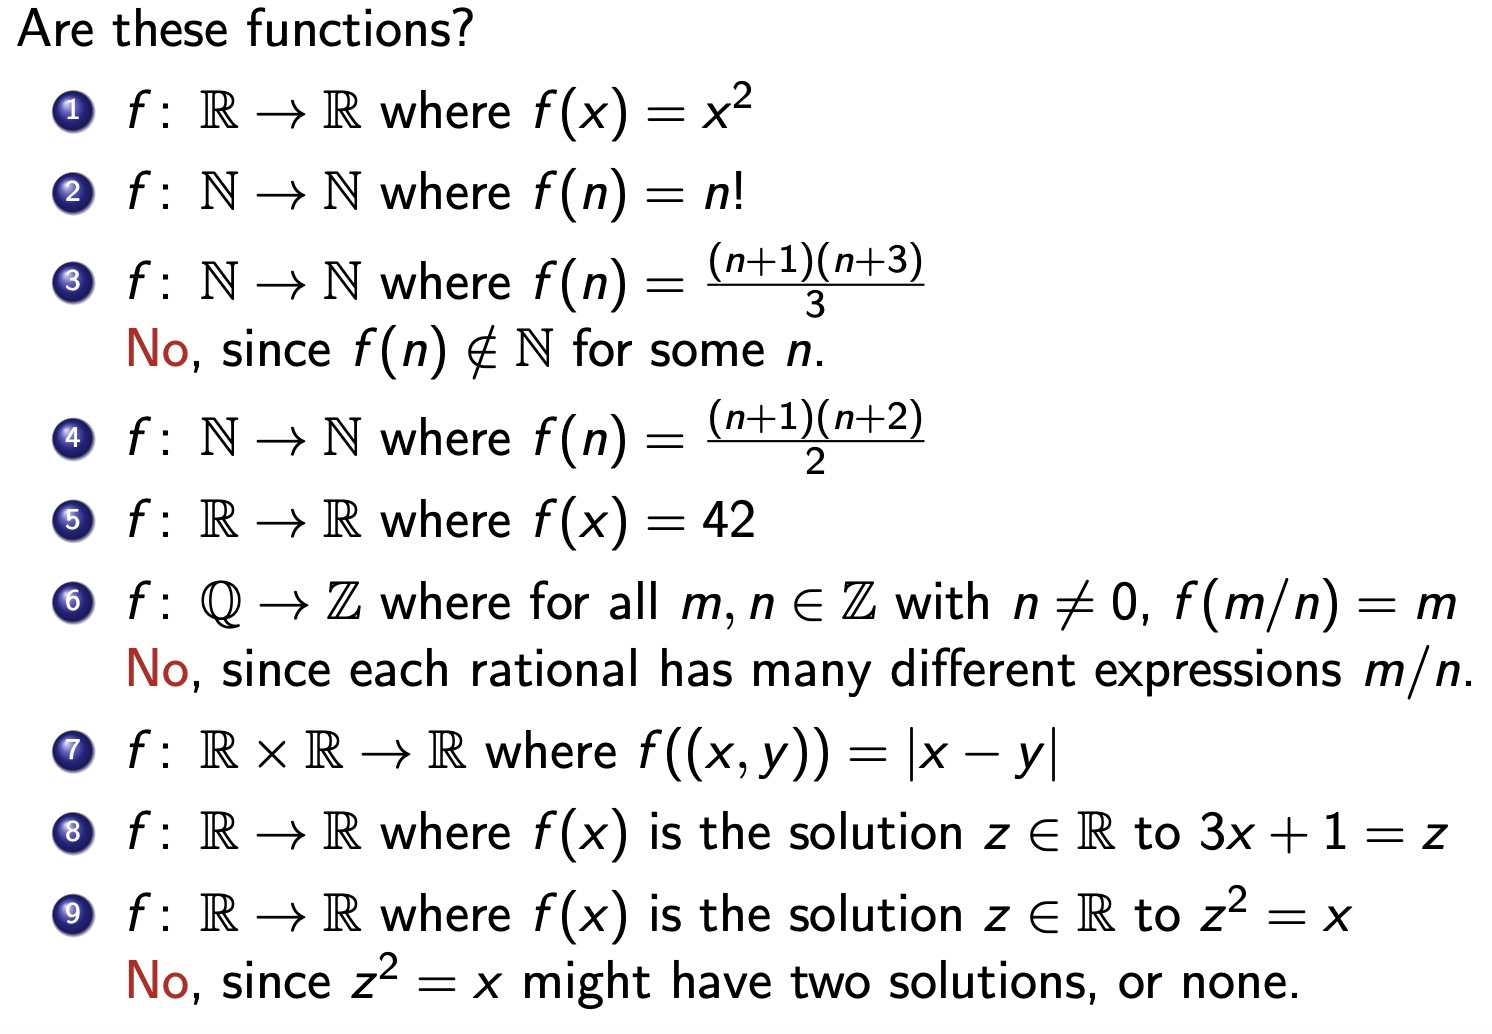
\includegraphics[width=0.6\linewidth]{graph/1.jpg} % 调整图片大小和图片路径
 \\
================================================================================================================
\newpage
================================================================================================================
\\
%========================================================================
\item Formal definition of funtion\\
We can think of a function as a subset of a Cartesian product:\\
A function $f : X \rightarrow Y$ is a subset $\neg \subseteq X \times Y$ such that, for each
$x \in X$, there is a unique $y \in Y$ such that $(x, y) \in \neg$. We write
$f(x)$ to denote this unique y.\\
Example: For $f: \mathbb{N} \rightarrow \mathbb{N}$ defined by $f(x) = x^2$\\
$\neg = \{(1,1),(2,4),(3,9),(4,16),......\}$\\
\\
The subset :\\
$\neg =\{(x,y) | x \in X \land f(x) = y\} \subseteq X \times Y$\\\\
is the graph of the function f. We have :\\
$\neg = \{(x,f(x)) | x \in X\} \subseteq X \times Y$\\

 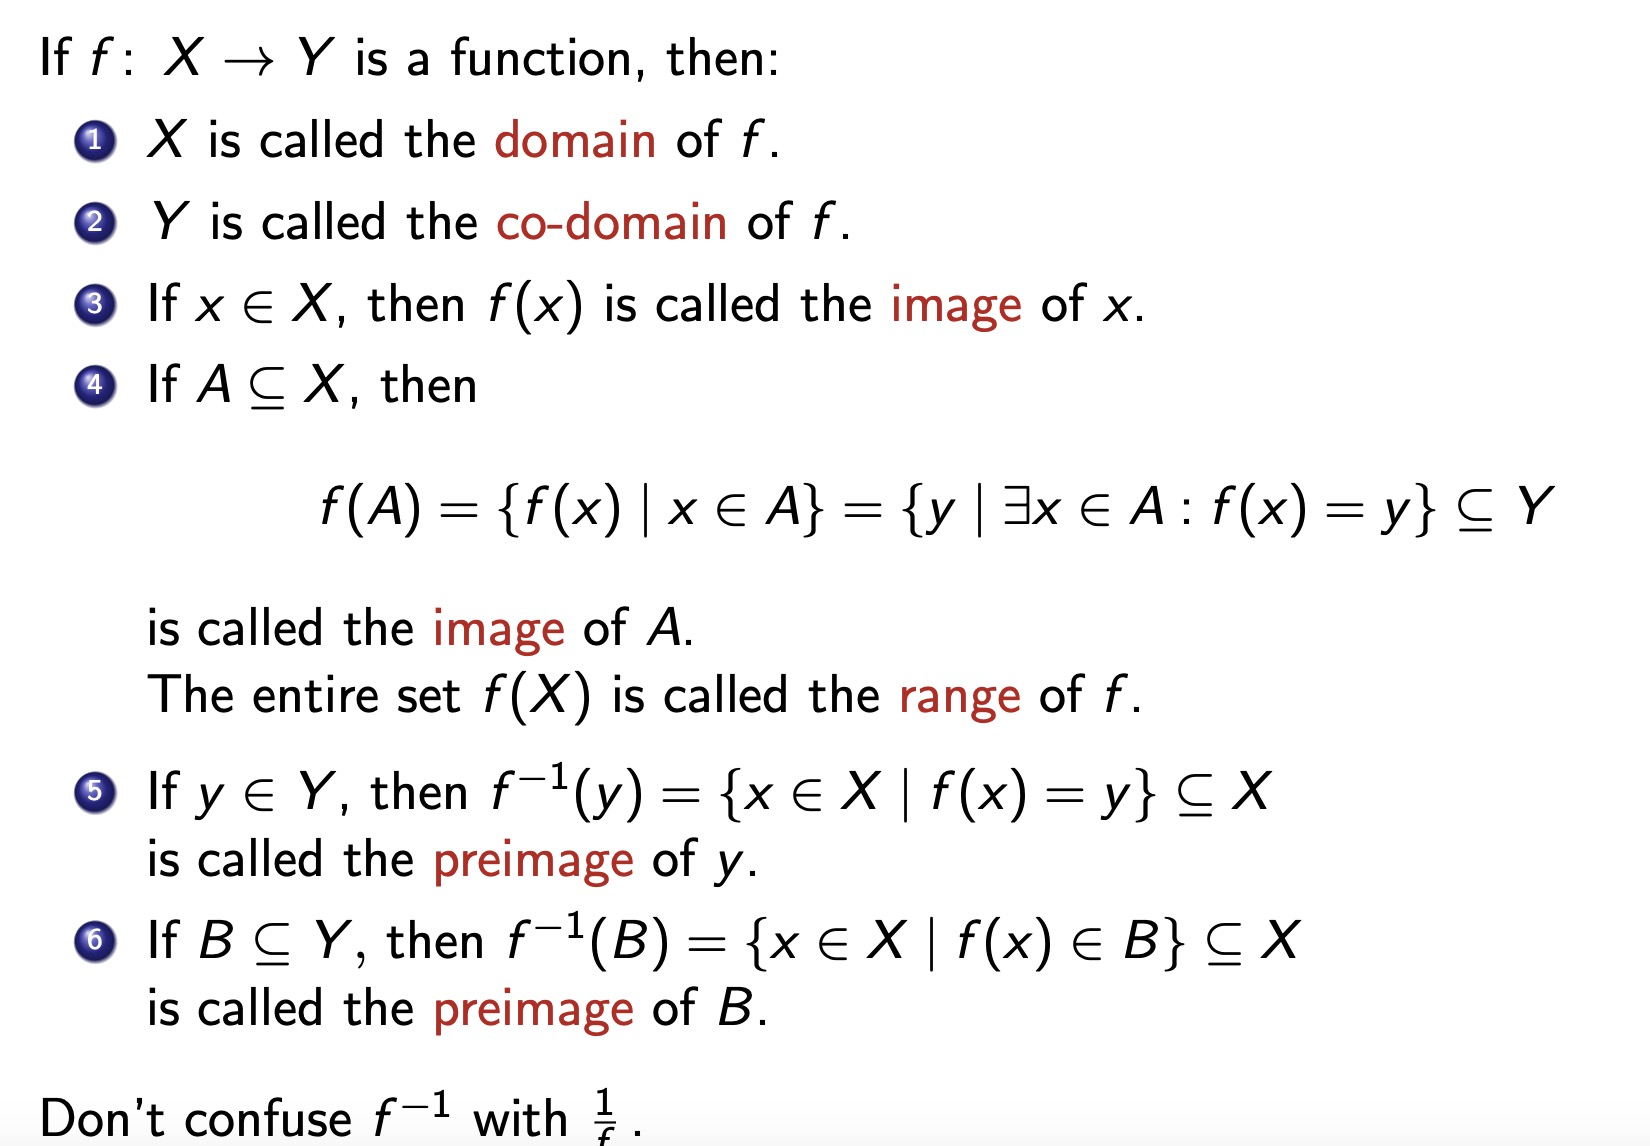
\includegraphics[width=0.8\linewidth]{graph/2.jpg} % 调整图片大小和图片路径
\\
================================================================================================================
\newpage
===============================================================================================================
\section{W4}

(i) Definitions
\item Equality of functions: \\
Functions $f , g : X \rightarrow Y$ are equal, written $f = g$, if and only if:\\
$f(x) = g(x) ,  \forall x \in X$\\
Note: $f$ denotes a function and $f(x)$ denotes an element of $Y$.\\\\
\textbf{Example}: $sin$ is a function; $sin(x)$ is just some number.

 %========================================================================
\item Floor :\\
Let $x \in \mathbb{R}$ be a real number. The floor of $x$, denoted $\lfloor x \rfloor$
 , is the unique integer n such that $n \leq x < n + 1$.
 %========================================================================
 \item Ceiling :\\
 Let $x \in \mathbb{R} $ be a real number. The ceiling of x, denoted $\lceil x \rceil$, is the unique
integer n such that $n-1 < x \leq n$.
 %========================================================================
\item Properties of functions \\
Let $f : X \rightarrow Y$ . Then:\\
\begin{itemize}

\item Surjective(onto) : 
$\forall y \in Y ,\exists x$ in $X$ such that $f(x) = y$\\Every element of Y is the image of something.

\item Injective(one - to- one):
$\forall x1,x2 \in X$,$f(x1) = f(x2) \rightarrow x1 = x2$\\Different elements of X have different images

\item Bijective
f is a one-to-one correspondence, or bijective, or a bijection, if f is
both one-to-one and onto.
The elements of X are “paired off” with the elements of Y\\

================================================================================================================
\newpage
================================================================================================================
 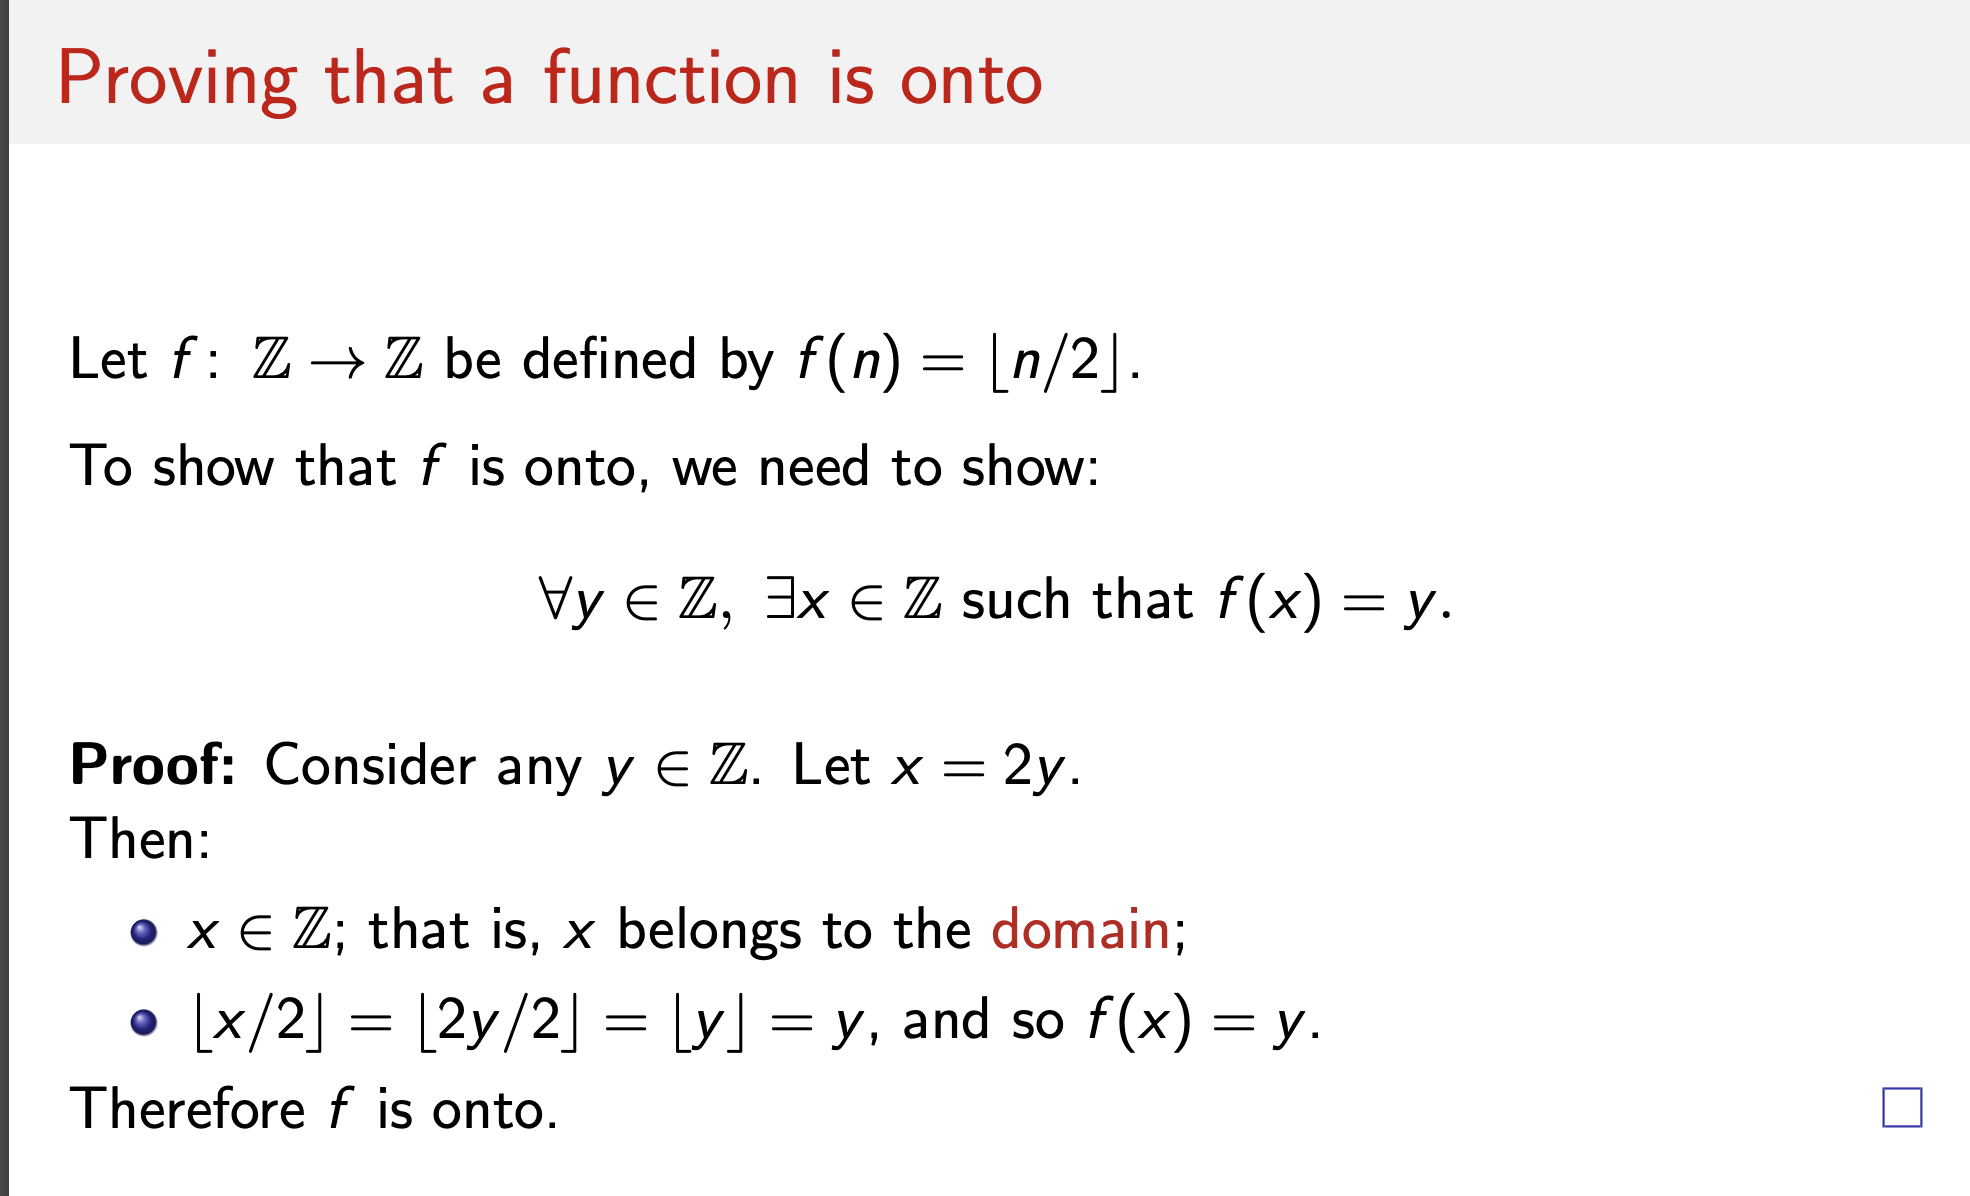
\includegraphics[width=1.0\linewidth]{graph/3.jpg} % 调整图片大小和图片路径
  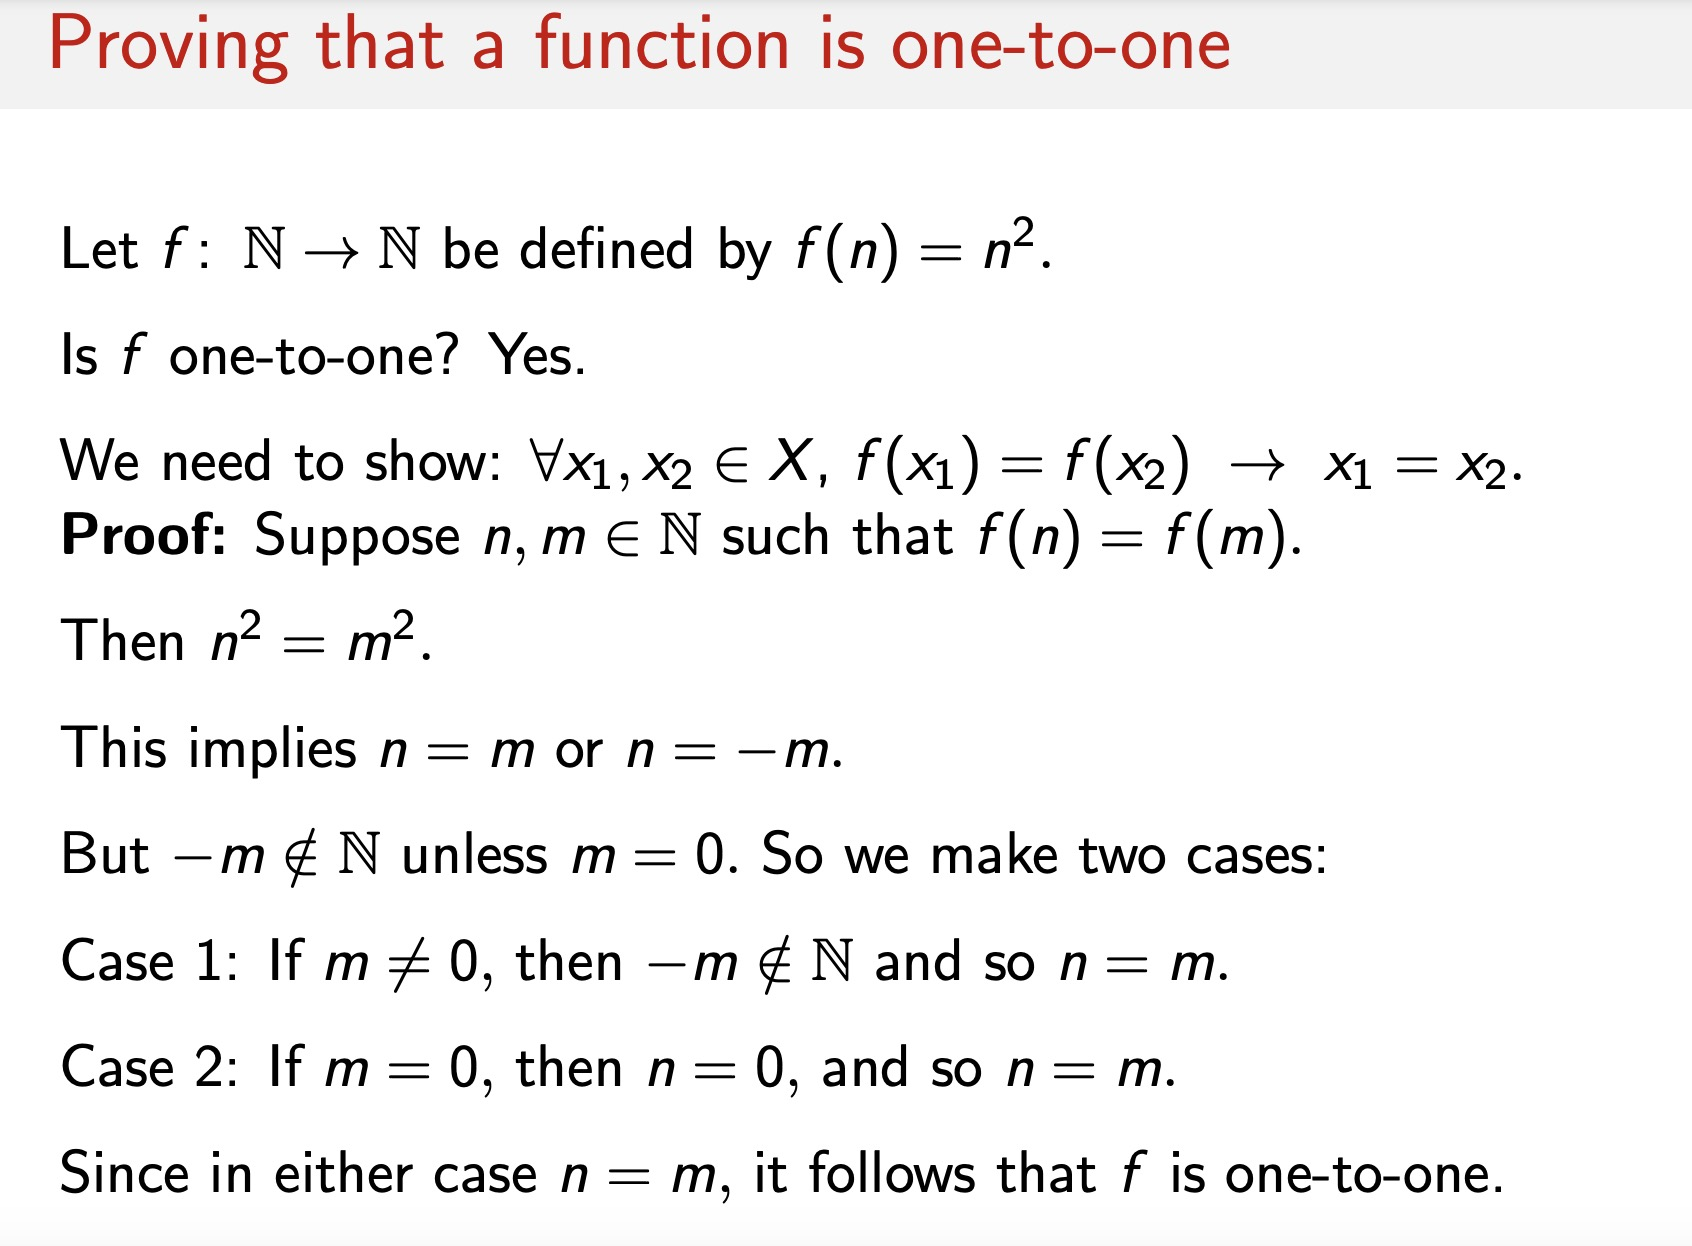
\includegraphics[width=1.0\linewidth]{graph/4.jpg} % 调整图片大小和图片路径
\end{itemize}
 %========================================================================
 
 ================================================================================================================
\newpage
================================================================================================================

\item Finite sets
Suppose X and Y are finite sets
\begin{itemize}
\item If $|X| > |Y|$, then there is no injective function $X \rightarrow Y$.
\item If $|X| < |Y|$, then there is no surjective function $X \rightarrow Y$.
\item There is bijective funtion $X \rightarrow Y$ if and only if $|X| = |Y|$
\end{itemize}
Put differently:
\begin{itemize}
\item If $f : X \rightarrow Y$ is injective , then $|X| \leq |Y|$. 
\item If $f : X \rightarrow Y$ is surjective ,then $|X| \geq |Y|$.
\item If $f : X \rightarrow Y$ is bijective ,then $|X| = |Y|$.
\end{itemize}
For finite sets with $|X| = |Y|$, the following statements
are equivalent:
\begin{itemize}
\item $f : X \rightarrow Y$ is injective
\item $f : X \rightarrow Y$ is bijective
\item $f : X \rightarrow Y$ is surjective
\end{itemize}
 
 %========================================================================
 \item Composition of functions
 If $f : X \rightarrow Y$ and $g : Y \rightarrow Z$, then the composition : \\
 $g \circ f : X \rightarrow Y$ is defined by:\\
 $(g \circ f)(x) = g(f(x)),\forall x \in X$
 
  %========================================================================
 \item Types of sequences
 Sequences can be finite:\\
 $5,5,20,5,5,60$ can be written as $(a_n)_{n=1}^6$ , where $a_1 = 5,a_2 = 5 . . . . . . a_6 = 60$\\
 or \hl{infinite}:\\
 $0,1,3,6,10,15,21 .. .. ....$ can be written as $(g_n)_{n \geq 0}$ where $g_0 = 0,g_1 = 1 ......$\\\\
 The index (the subscript) does not need to start at 0, and does not need
to be called n:\\
$1,5,15,35,70......$ can be written as $(f_i)_{i \geq 4}$,where $f_4 = 1,f_5 = 5, f_6 =15$ and so on\\
An alternating sequence alternates between positive and negative:\\
$((-\frac{1}{2})^n)_{n \geq 0} = 1, -\frac{1}{2},\frac{1}{4},-\frac{1}{8}, ......$
  %========================================================================
  
\item Define a sequence recursively
\begin{itemize}
\item Initial conditions, which directly specify one or more terms that begin
the sequence:\\
$F_0 = 0,F_1 = 1$\\
\item A recurrence relation, which defines every other term using earlier
terms:\\
$F_n = F_{n-1} + F_{n-2} $ for $n \geq 2$
\end{itemize}

================================================================================================================
\newpage
================================================================================================================
 %========================================================================
 \item Notation for sums:
 For a sequence $(a_i)$, we can add some or all of its terms:\\
 
$\sum_{i = m}^n a_i$ = $a_m + a_{m+1} + a_{m + 2} + ...... + a_n$\\

\textbf{Dummy variables}
The i in $\sum_{i = m}^n$ is a dummy variable, like the x in $\forall x$\\
\begin{itemize}
\item You can use any letter here (as long as it is not already taken):
\item The dummy variable is only relevant inside the sum, which means you can
reuse it outside the sum:\\
$\sum_{i = 1}^3 i + \sum_{i = 1}^4 i^2$ = $1+2+3+1+4+9+16$
\item You can also perform a change of variable. If k = i + 1, then:\\
$3! + 4! + 5!$ = $\sum_{i = 3}^5 i!$ = $\sum_{k = 4}^6 (k - 1)!$
\end{itemize}
 
 %========================================================================
 \item Arithmetic with finite sums
\begin{itemize}
\item Adding / subtracting over the same range:\\
$\sum_{i = m}^n a_i \pm \sum_{i = m}^n b_i$ = $\sum_{i = m}^n (a_i \pm b_i)$

\item Taking out a common factor:\\
 $\sum_{i = m}^n ca_i$ =  $c \sum_{i = m}^n a_i$
 
 \item Combining consecutive indices:\\
 $\sum_{i = p}^q a_i$ + $\sum_{i = q+1}^r a_i$ = $\sum_{i = p}^r a_i$,  if $p \leq q \leq r$
 
 \item Index shift:\\
 $\sum_{i = m}^n a_i$ =  $\sum_{i = m+p}^{n + p} a_{i - p}$ 
 
 \item Telescoping sums:\\
  $\sum_{i = m}^n (a_i - a_{i+1})$ = $a_m - a_{n+1}$ if $m \leq n$
\end{itemize}
%========================================================================

\item Divisiblity\\
If $n,d \in \mathbb{Z}$,then n is divisible by d if and only if there exists some $k \in \mathbb{Z}$ such that $n = kd$ \\
We write $d \mid n$.We also say `d divides n` or `d is a divisor of n`.
	
%========================================================================
\item Lemma (Bounds for divisors)\\
Let $n,d \in \mathbb{Z},$ If $|n| > 1$ and $d \mid n$, then $0 < |d| \leq |n|$.\\
Proof of lemma: Suppose $n,d \in \mathbb{Z}$ with $|n| \geq 1$ and $d \mid n$.Then there is some $k \in \mathbb{Z}$ such that $n = kd$.\\

The key steps in this proof were to:
\begin{itemize}
\item prove $0 < |d|$ by contradition
\item prove $|d| \leq |n|$ in the special case where $n, d \in \mathbb{N}$
\item reduce the general case $n, d \in \mathbb{Z}$ to an instance of our
special case.
\end{itemize}

%========================================================================
================================================================================================================
\newpage
================================================================================================================

\item The Quotient-Remainder Theorem
Given any integer n and positive integer d,\\
there exist unique integers q and r such that:\\
$n = q(quotient)*d(divisor) + r(remainder)$ and $0 \leq r < d$\\
We call q the \hl{quotient}, and r the \hl{remainder}.

%========================================================================
\item Modular arithmetic:\\
If n and m leave the same remainder after division by d,
we say that they are \hl{congruent modulo} d.\\
We write: $n \equiv m$(mod d)\\
If $n \equiv m$ (mod d), then $m \equiv n$ (mod d).
So the relationship is \hl{symmetric}.\\

If $a \equiv b$(mod d) and $n \equiv m$(mod d),then
\begin{itemize}
\item $an \equiv bm$(mod d)
\item $a+n \equiv b+m$(mod d)
\item $a-n \equiv b-m$(mod d)
\end{itemize}

%========================================================================


================================================================================================================
\newpage
================================================================================================================

\section{W5}

\item \textbf{Prime factorisation} : \\
The natural number $n \in \mathbb{N}$ is said to be writthen as a \hl{product of primes} if there is a natural number $m \in \mathbb{N}$ and prime numbers $p_1,......,p_m$ such that:\\
\textbf{$n = p_1 * p_2 * ... * p_n = \Pi_{k=1}^m p_k$}\\
\textbf{every natural number $n>1$ can be written as a product of primes.}

\item The fundamental Theorem of Arithmetic\\
Given any integer $n > 1$,there exists a natural number k ,pairwise distinct prime numbers $p_1,p_2,......,p_k$,
and natural numbers $e_1,e_2,....,e_k$ such that:
\textbf{$n = p_1^{e_1} * p_2^{e_2} *......*p_k^{e_k} = \Pi_{i = 1}^k p_i^{e_i}$}\\
\textbf{and any other expression for n as a product of prime numbers is identical to this except possibly for the order in which the factors are written.}

\item greatest common divisor of two integers a and b(\hl{not both zero})is the largest $d \in \mathbb{N}$ for which $d | a$ and $d | b$

\item least  common mutiple of two \hl{positive} integers a and b is the smallest $n \in \mathbb{N},n > 0$,for which $a | n$ and $b | n$ (we exclude zero here because this is always a solution).

\item compute gcd without prime factorisation:\\
\hl{$\forall a,b \in \mathbb{Z},gcd(a,b) = gcd(b,a-b)$}.
Why?
\begin{itemize}
\item if $d | a$ and $d | b$, then $d | a-b$
\item if $d \ b$ and $d | a-b$,then $d | b + (a - b) = a$
\end{itemize}

So: the common divisors of a and b are the \hl{same} as the common divisors of  b and a-b.\\
In particular, the \hl{greatest} common divisor of a and b is the same as the greatest common divisor of b and a - b.\\
\hl{\textbf{Speed way:$\forall a,b \in \mathbb{Z}$, if $a = bq + r$,then gcd(a,b) = gcd(b,r)}}

================================================================================================================
\newpage
================================================================================================================

\item \textbf{The Euclidean algorithm}\\
To find gcd(a,b) where $a,b \in \mathbb{Z}$ and $ a \geq b > 0$
\begin{itemize}
\item Write $a = qb + r$ as in the quotient-remainder theorem
\item if r=0, then terminate with gcd(a,b) = b
\item otherwise, replace (a,b) by (b,r) and repeat
\end{itemize}
\hl{Notice that the gcd is the last none-zero remainder.}\\

We've only discussed $a,b \geq 0$.What about arbitrary $a,b \in \mathbb{Z}$?
\begin{itemize}
\item If one or both of a,b are negative, then just ignore the negative signs: $gcd(a,b) = gcd(|a|,|b|)$
\item if a=0 and b=0, then gcd(a,b) is not defined
\item if a $\neq$ 0 and b=0 , then gcd(a,b) = $|a|$.
\item if a = 0 and b $\neq$ 0 , then gcd(a,b) = $|b|$.
\end{itemize}

\item Representation of integers(Base b expansion):\\
Let b be an integer greater than 1.Every positive integer n can be expressed uniquely in the form:\\
$n = a_kb^k + a_{k-1}b^{k-1} + ... + a_1b + a_0$\\
where k is a none-negative integer, $a_0,...,a_k$ are none-negative integers less than b and $a_k \neq 0$

\item O-notation:\\
O-notation is a mathematical notation that describes \hl{how quickly a
function f grows} compared to some function g when both their arguments
tend towards infinity.\\
For a given g it assigns a (large) set of functions which all grow at roughly
the same rate, or slower. The comparison is done by checking whether f is
an element of this set.\\
\hl{Definition}:

Let f and g be functions from a subset $A \in \mathbb{R}$ to $\mathbb{R}$. Then f (x) is in
O(g(x)) if there exist constants C and k such that for all $x \in \mathbb{A}, x \geq k$:
\begin{center}
$|f(x)| \leq C |g(x)|$
\end{center}

\textbf{For this to make sense $f$ must have the following properties}\\
\begin{itemize}
\item $f,g : A \subset \mathbb{R} \rightarrow \mathbb{R}$
\item A is unbounded(for all $k \in A$ there exist infinitely many $x \in \mathbb{A} $such that $ x \geq k$)
\end{itemize}

================================================================================================================
\newpage
================================================================================================================

\hl{Operations}
\begin{itemize}
\item $f(n) \in O(f(n))$
\item $O(c \cdot f(n)) = O(f(n))$ if c is a \hl{constant}
\item $O(f(n) + f(n)) = P(f(n))$
\item $O(f(n)g(n)) =f(n) \cdot O(g(n))$
\end{itemize}
\hl{Note}: Here, we use '=' to mean set equality\\

\hl{Important examples}\\
  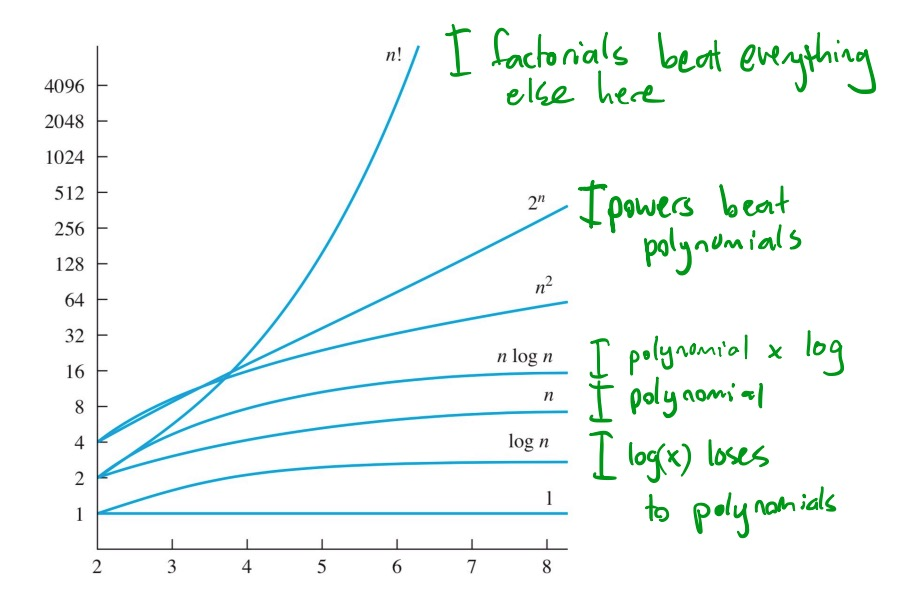
\includegraphics[width=1.2\linewidth]{graph/7.jpg} % 调整图片大小和图片路径
================================================================================================================
\newpage
================================================================================================================

\item Lower bound and exact order\\

Definition [$\Omega -notation$]:Let f and g be functions from a subset $A \in \mathbb{R} to \mathbb{R}$.Then f(x)
is in $\Omega(g(x))$ if there are positive constants C and k such that for all $x \geq k$:

\begin{center}
$|f(x)| \geq C|g(x)|$
\end{center}

Definition [$\Theta -notation$]:let f and g be functions from asubset $A \in \mathbb{R} to \mathbb{R}$. Then f(x) is in $\Theta(g(x))$ if $f(x) \in O(g(x))$ and $f(x) \in \Theta(g(x))$.\\
\hl{f(x) is $\Theta(g(x))$ means that f(x) and g(x) are of the same order(within a constant of each other)}.


================================================================================================================
\newpage
================================================================================================================
%========================================================================
\section{W6}

\item \textbf{Number of operations: Best-case, worst-case, average-case}\\\\
  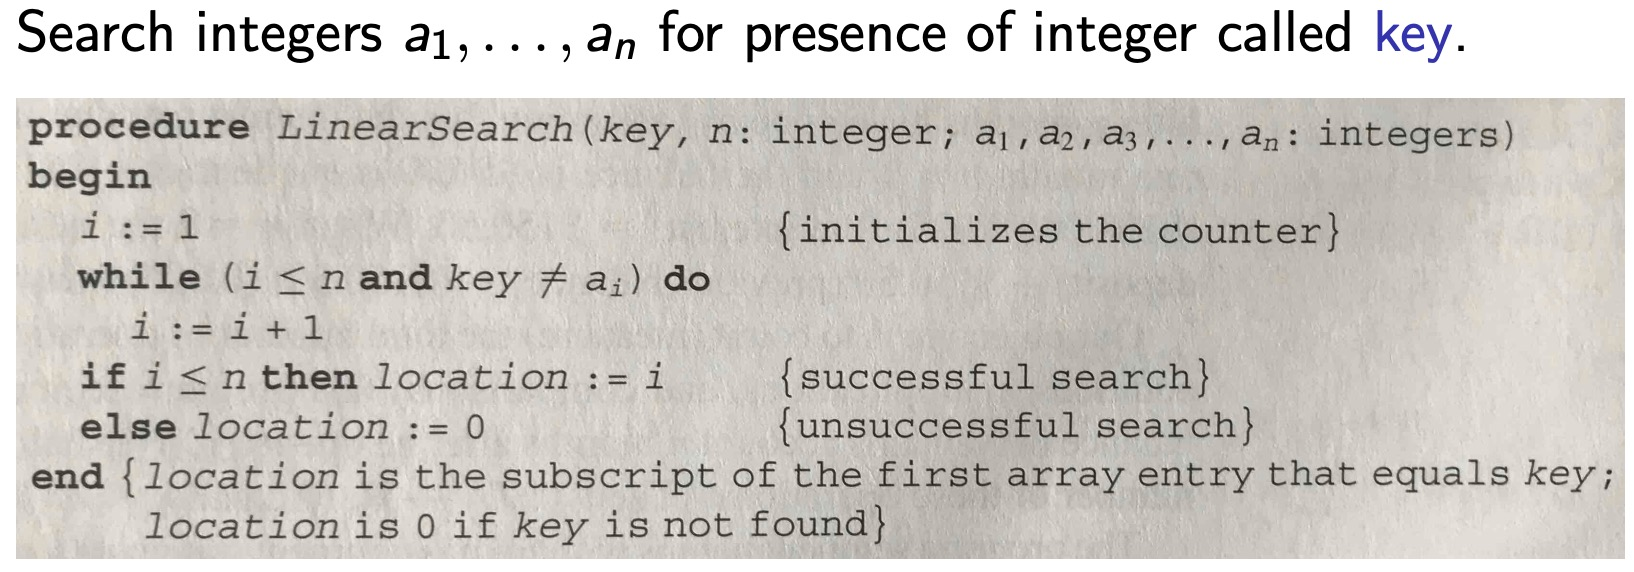
\includegraphics[width=1.0\linewidth]{graph/5.jpg} % 调整图片大小和图片路径
  
\begin{itemize}
\item Best-case scenario: $key = a_1$, complexity of algorithm is O(1) ,  O(n) (in fact, $\Theta(nx)$).
\item Worst-case scenario: $key =  a_n$, complexity of algorithm is O(n)
\item Average scenario : Assume key is in the list and equal to $a_k$ with probability p = 1/n\\
$f(n) = 1*p + 2*p + 3*p +......+ n*p = (n + 1)/2$
\end{itemize}
  
 \item \textbf{Number of operations: Euclidean algorithm}\\\\
  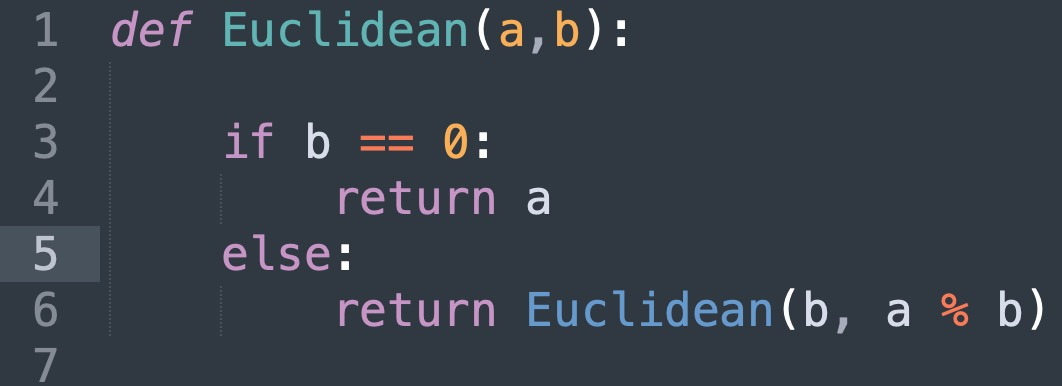
\includegraphics[width=1.0\linewidth]{graph/6.jpg} \\% 调整图片大小和图片路径
  \textbf{INPUT}: 2 none negative integers\\
  \textbf{OUTPUT}: gcd(a,b)\\
  
 A call of Euclidean has 
 \begin{itemize}
 \item 2 operations if b = 0 (check b , return a)
 \item 3 operations if b $>$ 0 (check b,a mod b,return function output)
 \end{itemize}


================================================================================================================
\newpage
================================================================================================================

How many steps are necessary until b = 0?\\
\hl{Idea: look at first argument every second step}
 \begin{itemize}
\item $r_i = k \cdot r_{i+1} + r_{i+2}$
\item $k \geq 1$
\item $r_i = k \cdot r_{i+1} + r_{i+2} \geq r_i = r_{i+1} + r_{i+2} > 2r_{i+2}$
\item $r_{i+2} < r_i / 2$
 \end{itemize}
 After at most \hl{2log2(a)} calls of Euclid, the arguments must be
gcd(a, b) and 0.\\

Running time: $3(2 log2(a)) - 1 \in O(log(a))$.
\item \textbf{Mathmatical induction}\\
Let P(n) be a predicate that is defined for all integers $n \geq a, a \in \mathbb{N}$, Suppose:
 \begin{itemize}
\item P(a) is true
\item For all integers  $n \geq a, P(n) \rightarrow P(n+1)$
 \end{itemize}
 Then P(n) is true for all integers $n \geq a$(\hl{We just assume P(n),we never directly proof P(n) is true})
 
\item \textbf{How to use mathematical induction}
 \begin{itemize}
\item Prove P(a) (\hl{This is called basic step})
\item Prove that for all integers  $n \geq a, P(n) \rightarrow P(n+1)$\\
(i) Assume P(n) is true for some particular but arbitrary $n  \geq a$;\\
(ii) using this, show that P(n + 1) is also true.\\
This is called the \hl{inductive step}.
The assumption that P(n) is true is called the
\hl{inductive hypothesis}.
 \end{itemize}


================================================================================================================
\newpage
================================================================================================================

\section{W7}

\item Case1 : \textbf{Order matters, repetition allowed} \\
If a decision process can be broken down
into a finite number of independent steps,
and there are ni possible outcomes for the ith step,
then the entire process can be carried out in $\Pi {ni}$ possible ways.\\
In particular: for finite sets $S_1,S_2,....S_k$,
\begin{center}
$|S_1 * S_2 * ... * S_k| = \Pi_{i=1}^k |S_i|$
\end{center}
\item Case2 : \textbf{Order matters, repetition not allowed}\\
If you choose k elements from a set S with n elements,
and order matters and repetition is not allowed,
then there are:
\begin{center}
n possiblities for the first choice,
then n - 1 for the second,
then n - 2 for the third,
...
then n - k + 1 for the kth.
\end{center}
So the total number of choices is :
\begin{center}
$n \cdot (n-1) \cdot (n-2) ... (n - k + 1) = \frac {n!} {(n-k)!}$
\end{center}

\item Case3: \textbf{ Order does not matter, repetition not allowed}\\

\begin{center}
$\frac {n!} {k!(n-k)!}$
\end{center}

\item Case4 : \textbf{Order does not matter, repetition allowed}\\
Choosing k items from a set of n items
such that order does not matter and repetition is allowed
is the same as \hl{counting all possible arrangements of k crosses and n  1 bars,
and this number is}
\begin{center}
$\frac{(k + n -1)!} {k!(n-1)!}$
\end{center}
================================================================================================================
\newpage
================================================================================================================
\section{W8}

\item \textbf{The inclusion-exclusion principle}

\[
\begin{aligned}
\left| A_1 \cup A_2 \cup \ldots \cup A_n \right| = & \sum_{i=1}^{n} \left| A_i \right| \\
& - \sum_{1 \leq i < j \leq n} \left| A_i \cap A_j \right| \\
& + \sum_{1 \leq i < j < k \leq n} \left| A_i \cap A_j \cap A_k \right| \\
& \vdots \\
& + (-1)^{n+1} \left| A_1 \cap A_2 \cap \ldots \cap A_n \right|,
\end{aligned}
\]

where \( A_1, A_2, \ldots, A_n \) are the sets in question. The principle alternates between addition and subtraction to account for overcounting in the intersections of the sets.

\textbf{Example}:I have 10 students, and I wish to give back their marked quizzes.
If I give the quizzes to students at random (without asking for student
numbers, but ensuring that \hl{everybody receives a quiz}),
what is the probability that \hl{nobody} receives their own quiz?

\begin{itemize}
\item{Step1} Total permutations : $10!$
\item{Step2} Permutations of at least 1 student gets right quiz:\\
Assume $A_i$ is the set of all permutations that i student(s) get right quizes
Where at least one student gets the right exam :  \\$| A_1 \cup A_2 \cup ....  \cup A_{10}|$
\item Probability: $\frac{10! - | A_1 \cup A_2 \cup ....  \cup A_{10}|} {10!}$(using \hl{ inclusion-exclusion principle} to calculate)
\end{itemize}

\item \textbf{The generalised pigeonhole principle}\\
If you have n pigeons sitting in k pigeonholes, and if n $>$ k · m, then\hl{ at
least one of the pigeonholes} contains at least \hl{m + 1} pigeons.

\textbf{Example}:\\
Suppose we have n = 101 pigeons to fit into k = 20 holes.
Then, using the generalised pigeonhole principle with m = 5, we can
conclude that some hole contains $\geq 6$ pigeons.


================================================================================================================
\newpage
================================================================================================================

\item \textbf{Balanced String}\\
String means a sequence of brackets where \hl{order matters}\\
Balanced means that in each initial substring, there are no more “)”
than there are “(”\\
\textbf{Examples}: Let bn be the number of balanced strings on n left-brackets and n
right-brackets.
\begin{itemize}
\item $b_0= 1 $ 
\item $b_1= 1 $ ()
\item $b_2= 1 $ ()(),(())
\item $b_3= 5 $((())),(()()),(())(),()(()),()()() 
\end{itemize}


\item \textbf{Monotonic lattice paths}\\
Let’s count special paths on an n x n grid going from the bottom left
corner to the top right corner. Namely, paths that only step right or up,
and stay below the diagonal.Let $p_n$ be the number of such paths.
  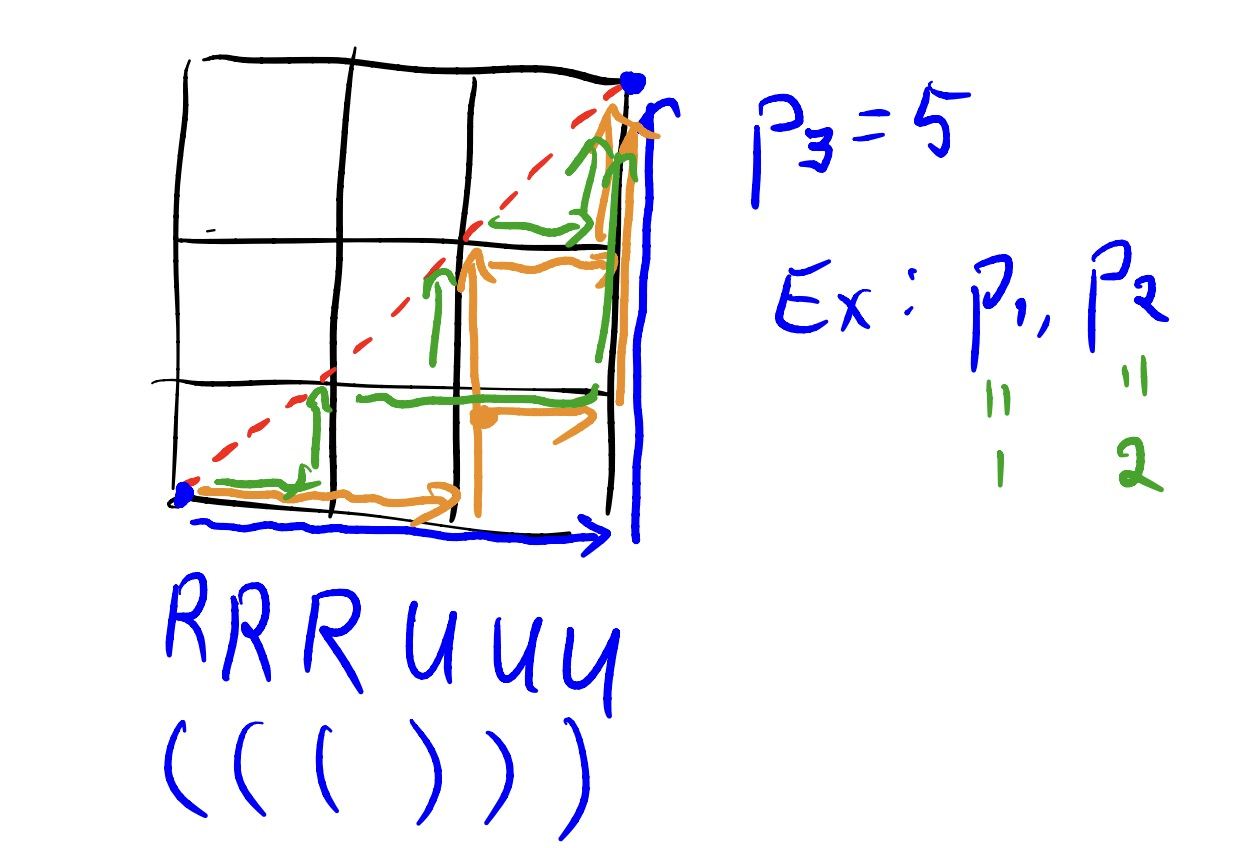
\includegraphics[width=1.0\linewidth]{graph/8.jpg} \\
  
Each monotonic lattice path is a sequence of n R’s and n U’s such that in
each initial subsequence there are no more U’s than R’s (since otherwise
the path would cross the diagonal).
We therefore have a well-defined map from monotonic lattice paths to
balanced strings defined by\\
$R \rightarrow ( $ and $L \rightarrow )$\\
This map is bijective, with inverse defined by\\
$( \rightarrow R$ and $) \rightarrow U$

================================================================================================================
\newpage
================================================================================================================

\item \hl{\textbf{Catalan Number} }
\begin{itemize}
\item \hl{Recurrence Relation:} $C_0 = 1, \quad C_{n+1} = \sum_{i=0}^{n} C_i \cdot C_{n-i} \text{ for } n \geq 0 $
\item \hl{Direct Formula:} $C_n = \frac{1}{n+1} \binom{2n}{n} = \frac{(2n)!}{(n+1)!n!}$
\end{itemize}

\item \hl{\textbf{Recurrences revisited}}\\
Consider a \hl{linear homogeneous} recurrence relation of order 2:
\begin{center}
$a_n = \alpha a_{n-1} + \beta a_{n-2}$
\end{center}

\textbf{method}
\begin{itemize}
\item {Step1} Factor $x_2 - \alpha x - \beta = (x - \alpha_1)(x - \beta_1)$
\item {Step2($\lambda_1 \neq \lambda_2$)}  then $a_n = A \lambda_1^n + B \lambda_2^n$
\item {Step2($\lambda_1 = \lambda_2$)}  then $a_n = C \lambda^n + Dn \lambda^n$
\end{itemize}

Solutions in (2a) and (2b) are the \hl{general solution} of the rec. relation.
\hl{Initial conditions} (values of $a_0$ and $a_1$) determine constants A, B or C, D.\\\\
\textbf{Eample}\\
Let $f : \mathbb{N} \rightarrow \mathbb{Z}$ be a function defined recursively by f(0) =-1, f(1) =5 and for all $n \geq 2$ by 
\begin{center}
$f(n) = 10 f(n-1) - 25 f(n-2)$
\end{center}

\begin{itemize}
\item {Step1} Factor $x_2 -10x + 25 = 0$
\item {Step2($\lambda_1 = \lambda_2 = 5$)}  then $f_n = A 5^n + B 5^n$
\item {Step3} $f(0)= A + 0 = -1$,$f(1) = -5^1 + B5^1 = 5 \rightarrow B = 2$
\end{itemize}

\textbf{\hl{linear non-homogeneous recurrence relation of order 2:}}
\begin{center}
$a_n = \alpha a_{n-1} + \lambda a_{n-2} + F(n)$
\end{center}

\textbf{method}
\begin{itemize}
\item {Step1} Find a paticular solution $a_n^{(p)}$ by \hl{poking around}
\item {Step2}  Determine the general solution $a_n^{(h)}$ to the homogeneous equation
\begin{center}
$a_n = \alpha a_{n-1} + \lambda a_{n-2}$
\end{center}
The general solution of the non-homogeneous recurrence relation is then
given by a $a_n^{(p)} + a_n^{(h)}$
\end{itemize}

When we are given initial conditions, i.e. values of a0 and a1, then these
determine the constants A, B or C, D.\\
================================================================================================================
\newpage
================================================================================================================

\textbf{Example}
\begin{center}
$a_n = 10 a_{n-1} - 25 a_{n-2} + 3^n$
\end{center}
From before, the homogeneous equation  $a_n = 10 a_{n-1} - 25 a_{n-2}$ has the  general solution $a_n^{(h)} = C \cdot 5^n +  D \cdot n5^n$ \\
\begin{itemize}
\item Try $a_n^{(p)} = E3^n$
\item $E3^n = 10E3^{n-1} - 25E3^{n-2 } + 3^n$
\item $E = \frac{9}{4}$
\end{itemize}

\textbf{solution} $a_h = a_n^{(h)} + a_n^{(n)}$ = $C \cdot 5^n + Dn5^n + 	\frac{9}{4} 3^n$


================================================================================================================
\newpage
================================================================================================================

\section{W9}
\item Setup
\begin{itemize}
\item \hl{Sample Space S} (also called \hl{probability space}). Here: $|S| < \infty $ 
\item $x \in S$ is called an \hl{outcome},or an \hl{elementary event}
\item $E \subseteq S$ is called an event
\item Set of events $\mathbb{E}$ is a subset of the power set of S, so $\mathbb{E} \subseteq P(S)$
\item For $x \in S$.\{x\} is called an \hl{elementary event}
\end{itemize}

\item Random A random variable is a function $X : S \rightarrow R$ defined on the outcomes of a
\hl{sample space}.\\
\textbf{Example}:\\S outcomes of the roll of two fair dice, so $|S| = 36$.
$X : S \rightarrow R,$ X(s) = “sum of the values of the two dice in outcome $s \in S$”
Then X(S) = \{2, 3, 4, 5, 6, 7, 8, 9, 10, 11, 12\}.

\item Distribution of random variable
\begin{center}
Set of all pairs (r, p(X = r) )
\end{center}
X refers to random variable which is a \hl{function} that assigns a real number to each outcome in a \hl{sample space}.

\item \textbf{\hl{Conditional probability}}
Let E and F be events with $p(F) > 0.$
The \hl{conditional probability} of E given F is
\begin{center}
$p(E | F) = \frac{p(E \cup F)}{p(F)}$
\end{center}

\textbf{Example}\\
In your local juggling club, 1/3
of all members are computer scientists.
Exactly 1/4 of all members pass clubs, 2/5
of these are computer scientists.\\
i) What is the percentage of computer scientists who pass clubs
amongst all members?\\
$p(E \cap F)$\\
ii) What is the percentage of computer scientists who pass clubs
amongst the computer scientists?\\
$p(F | E)$

\item \textbf{Independent}: If any of the following hold, E and F are called independent.(The following are \hl{equivalent})
\begin{itemize}
\item $p(E | F) = p(E)$
\item $p(E \cap F) = p(E)p(F)$
\end{itemize}


================================================================================================================
\newpage
================================================================================================================\\

 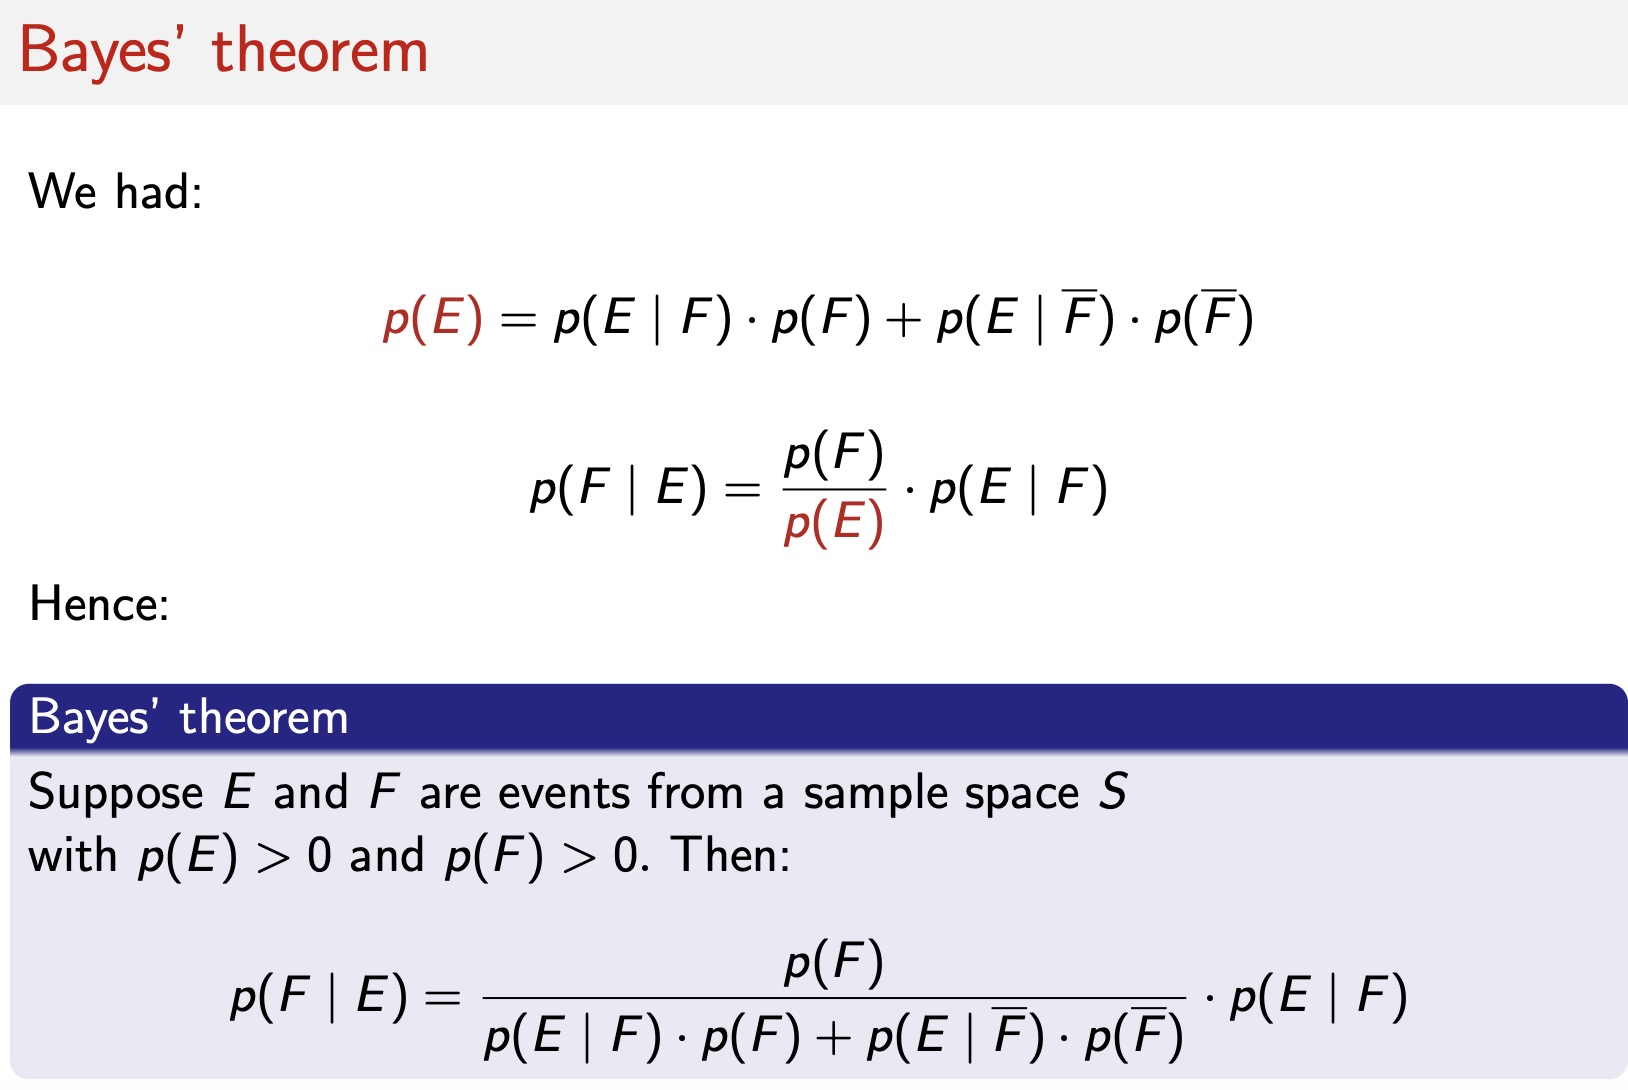
\includegraphics[width=1.0\linewidth]{graph/9.jpg} \\% 调整图片大小和图片路径
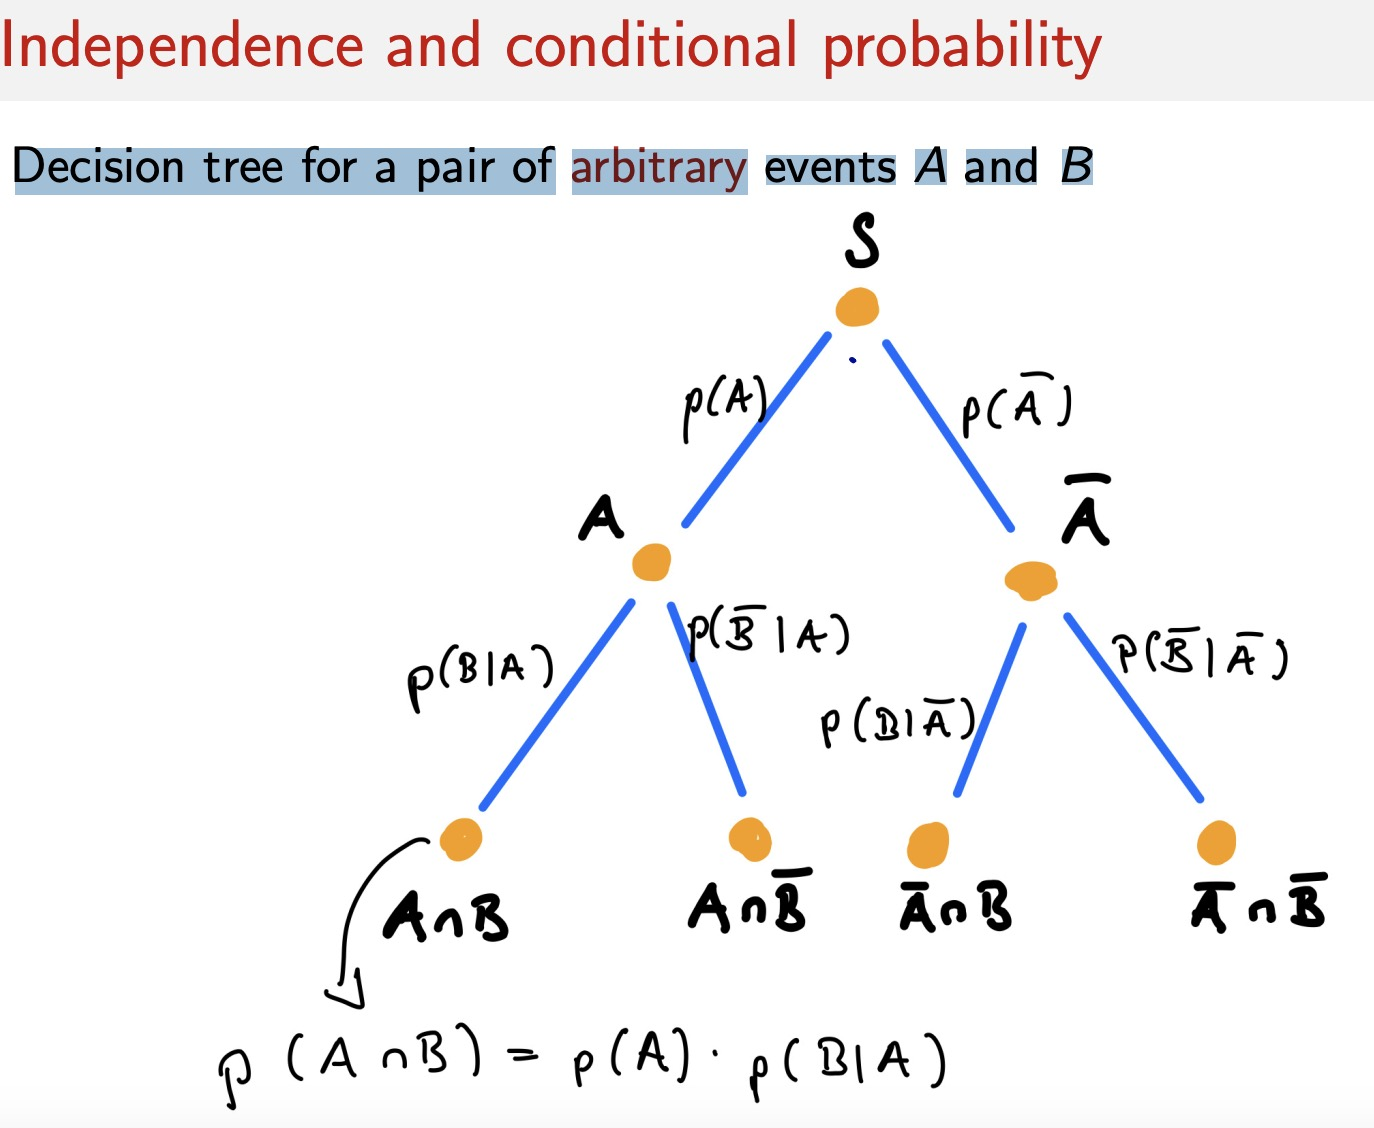
\includegraphics[width=1.0\linewidth]{graph/10.jpg} \\% 调整图片大小和图片路径
================================================================================================================
\newpage
================================================================================================================\\
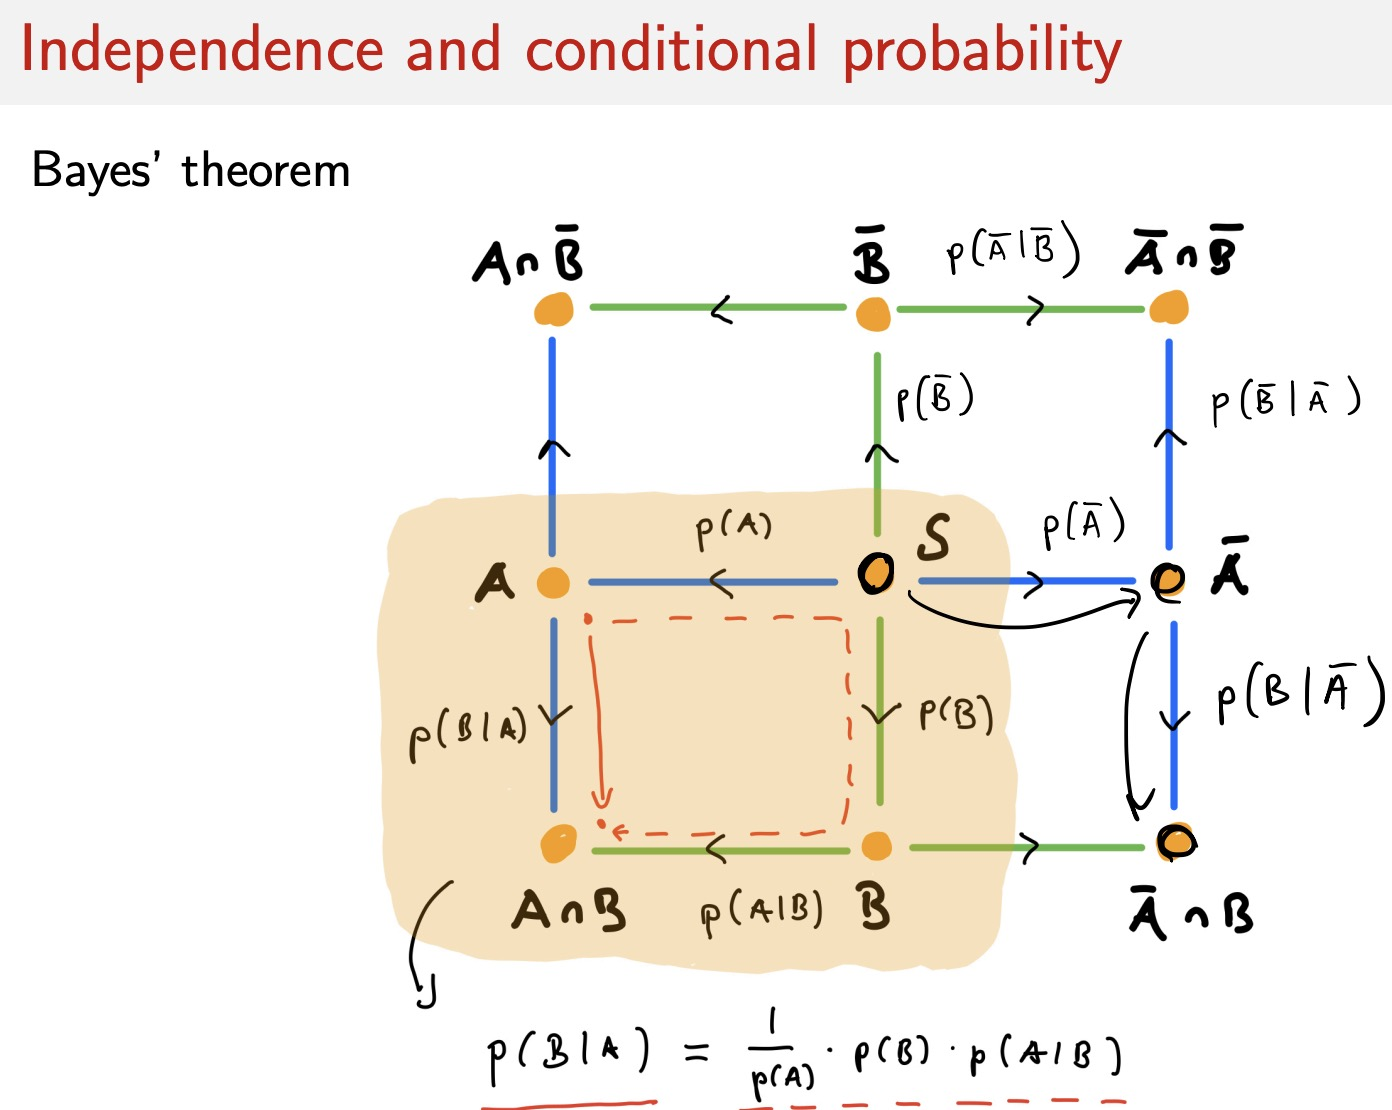
\includegraphics[width=1.0\linewidth]{graph/11.jpg} \\% 调整图片大小和图片路径
      



================================================================================================================
\newpage
================================================================================================================\\

\section{W10}
\item Relation

\begin{itemize}
\item Let X and Y be sets. A relation \hl{R} from X to Y is a subset of $X \times Y$
\item We write $(x, y) \in R$ also as \hl{$x R y$} and say that x is related to y.
\item The \hl{complementary relation} to R is $\overline{R} = (X \times Y) \backslash R$
\item If $X = Y$ we say that R is a relation on X.
\end{itemize}

\item  Properties\\
Let R be a relation on the non-empty set X. Then:
\begin{itemize}
\item Reflexive :  $\forall x \in X , (x,x) \in \mathbb{R}$
\item Symmetric : $(x,y) \in \mathbb{R}  \rightarrow (y,x) \in \mathbb{R}$
\item Transitive : $(x,y) \in \mathbb{R} \land (y,z) \in \mathbb{R} \rightarrow (x,z) \in \mathbb{R}$ 
\end{itemize}

\item Combining Relations\
The relations $R_1$ and $R_2$ from X to Y are a subsets of $ X \times Y $
We can use operations on subsets to create new relations:
\begin{itemize}
\item $R_1 \cup R_2$
\item $R_1 \cap R_2$
\item $R_1 \backslash R_2$
\end{itemize}

We can \hl{compose} relations R from X to Y and S from Y to Z to get a
new relation $S \circ R$ from X to Z by defining:
\begin{center}
$S \circ R = \{(a,c) | \exists b \in Y : aRb \land bSc \subseteq X \times Y\}$
\end{center}

\item Equivalence relation
If the relation R on the non-empty set X is \textbf{reflexive, symmetric and
transitive}, then R is an \hl{equivalence relation} on X.

\item Equivalence class\\
If R is an equivalence relation on X and $x \in X$ then the set
\begin{center}
$[x] = \{y \in X | (x,y) \in R\}$
\end{center}
is the \hl{equivalence class} of x.\\

================================================================================================================
\newpage
================================================================================================================\\

\textbf{Example}\\
$(m,n) \in R$ if and only if $3 | (m - n)$
these are 3 equivalence classes
\begin{itemize}
\item $\{..., -6, -3, 0, 3, 6,...\}$
\item $\{..., -5, -2, 1, 4, 7,...\}$
\item $\{..., -4, -1, 2, 5, 8,...\}$
\end{itemize}
We can (if we like) call these [0], [1] and [2].\\\\
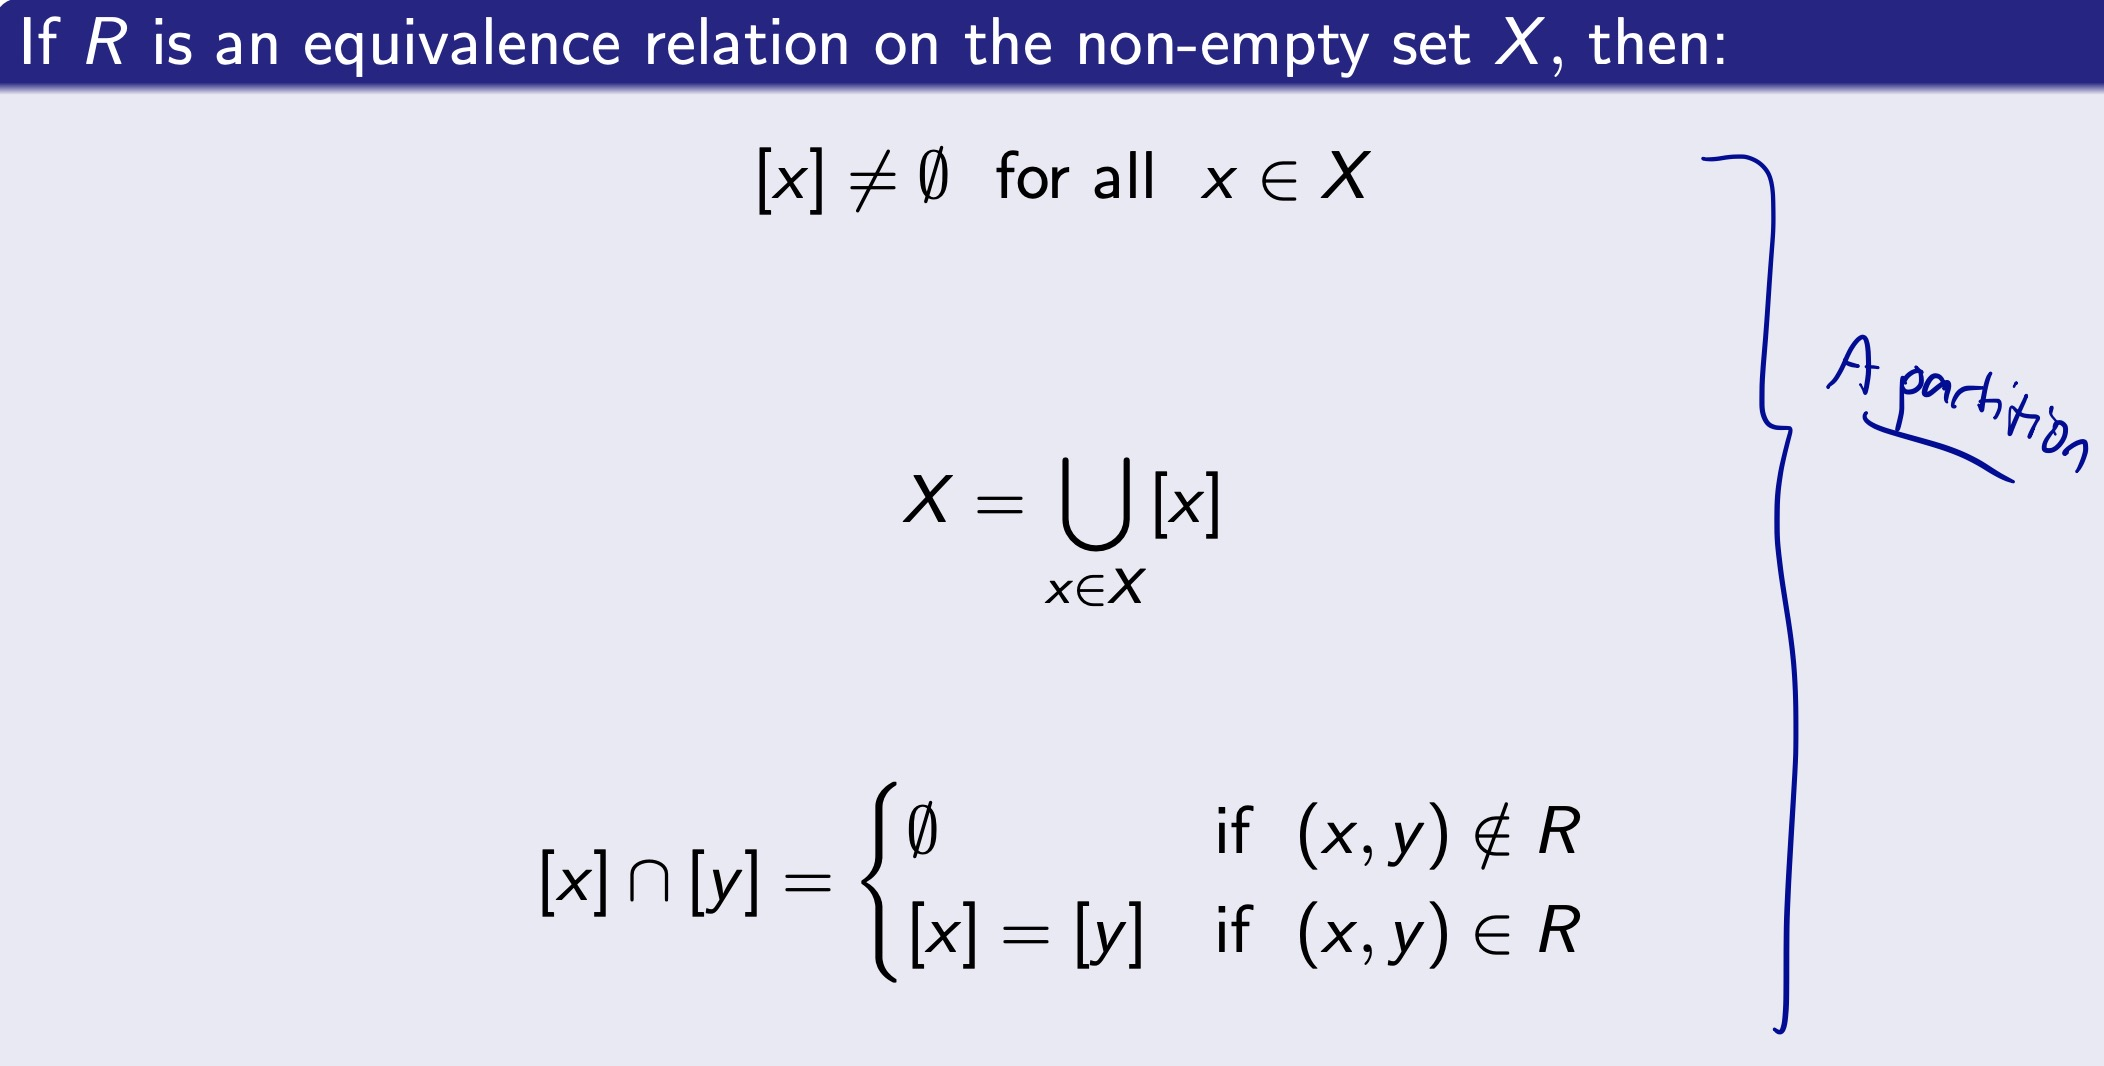
\includegraphics[width=1.0\linewidth]{graph/12.jpg} \\% 调整图片大小和图片路径

================================================================================================================
\newpage
================================================================================================================\\

\item Partition\\
A set $\{S1, S2,...\}$ is a partition of S if:
\begin{itemize}
\item $S_i \neq \emptyset$
\item $S = S_1 \cup S_2 \cup .. ....  S_i$ \qquad The sets cover S
\item $S_i \cap S_j = \emptyset$ whenever $i \neq j$ \qquad The sets are disjoint
\end{itemize}

\hl{An equivalence relation on X gives a partition of X}\\
\hl{A partition of X gives an equivalence relation on X.}\\
\\
Suppose $\{X_1, X_2,...\}$ is a partition of X.
Then the relation $R$ defined by
\begin{center}
$xRy \leftrightarrow \exists i$ such that $x \in X_i$ and $y \in X_i$
\end{center}
is an equivalence relation.\\
In other words : \textbf{If two elements belong to the same subset, then they are related.}

\item Anti-symmetric\\
The relation R is anti-symmetric if and only if :
\begin{center}
$\forall a,b \in X,  (a,b) \in R$ and $(b,a) \in R$ implies $a=b$\\
\end{center}

\begin{itemize}
\item \hl{can not} have both (1,3) and (3,1)
\item may not have either
\item anti-symmetric $\neq$ not symmetric\\
\textbf{Example}: symmetric and anti-symmetric
\hl{$\{(1,1),(2,2),(3,3)\}$}
\end{itemize}

\item Partial and total orders\\
A relation R on a set X which is \hl{reflexive, transitive, and anti-symmetric} is
called a partial order on X.
If in addition, $\forall a,b \in X$,$aRb$ or $bRa$, then R is called a \hl{total order} on X.\\
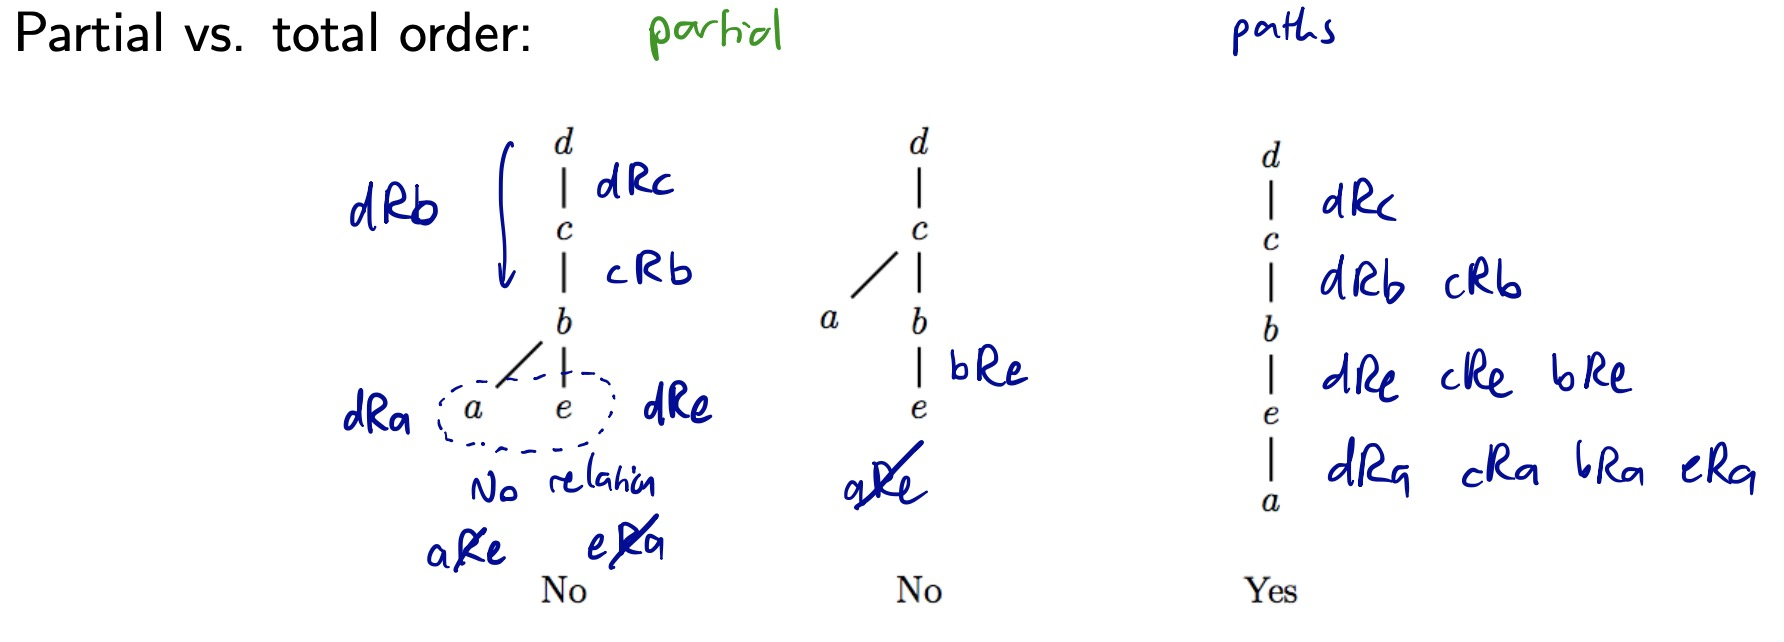
\includegraphics[width=0.8\linewidth]{graph/13.jpg} \\% 调整图片大小和图片路径


================================================================================================================
\newpage
================================================================================================================\\

\item Reflexive closure\\
$ref(R) = R \cup \{(x,x) | x \in X\}  =R \cup \Delta$\\
For a digraph representation: \hl{add a loop} at each vertex\\
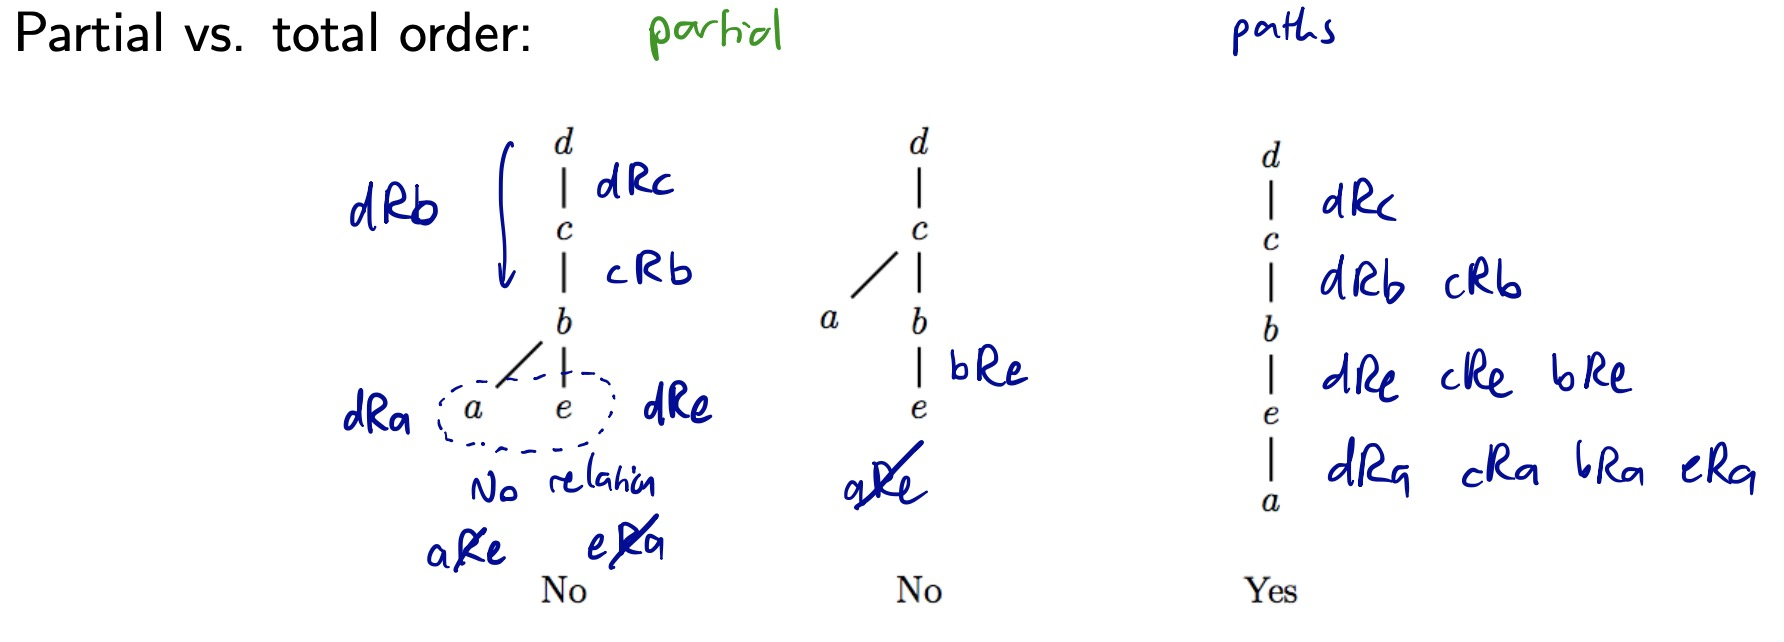
\includegraphics[width=1.2\linewidth]{graph/13.jpg} \\% 调整图片大小和图片路径

\item Symmetric closure\\
$R \cup \{(y,x) | (x,y) \in R\} = R \cup R^{-1}$\\
For a digraph representation: \hl{Add edges in the opposite direction}\\
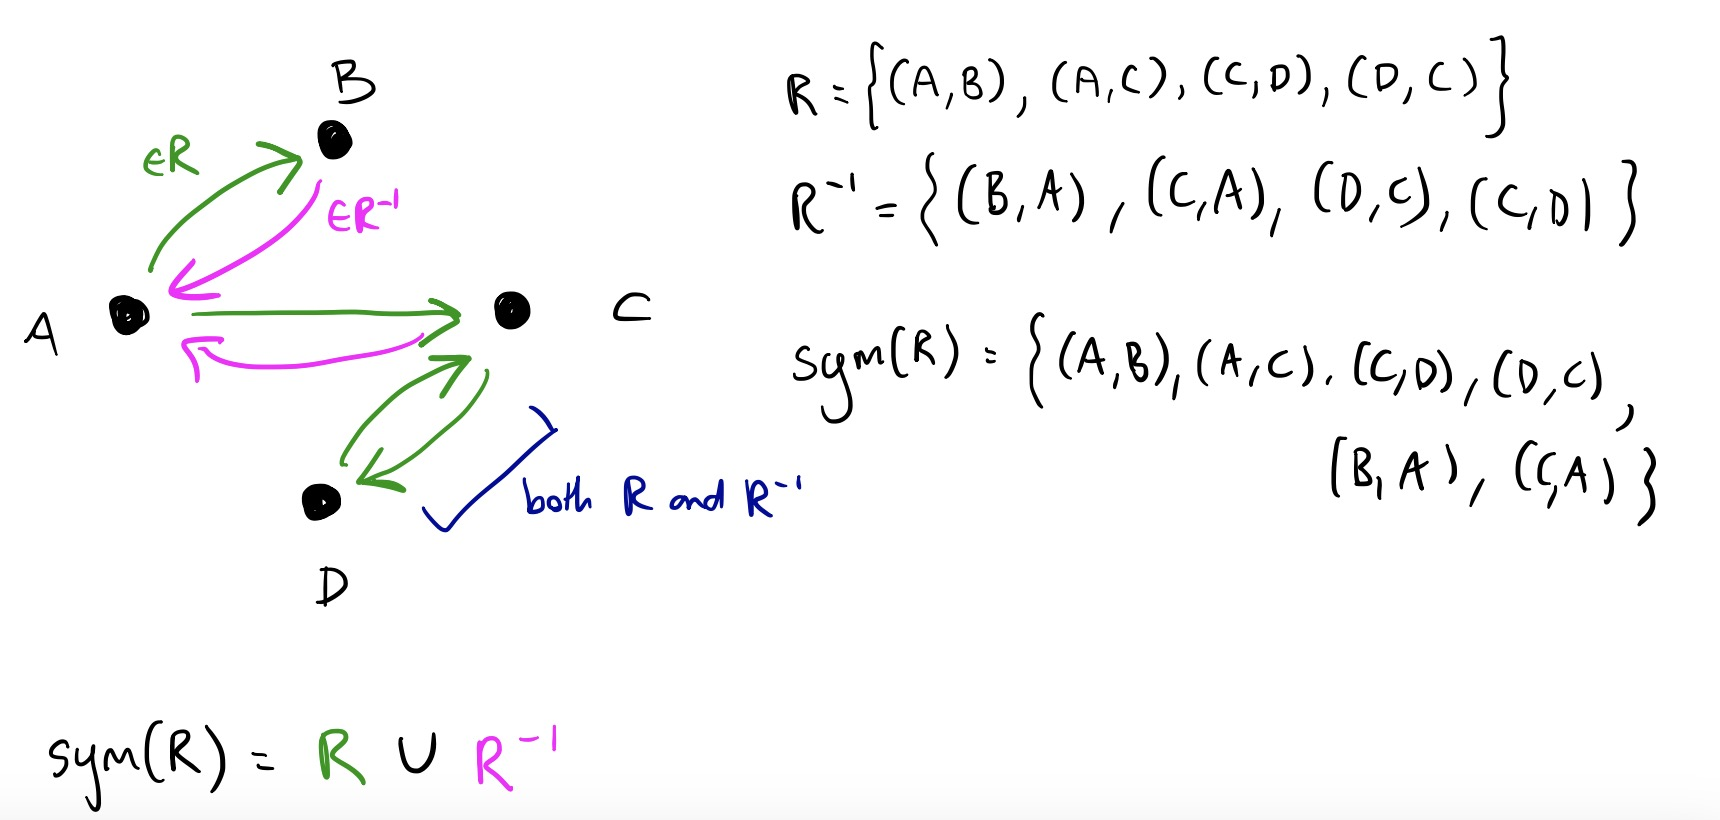
\includegraphics[width=1.2\linewidth]{graph/15.jpg} \\% 调整图片大小和图片路径

================================================================================================================
\newpage
================================================================================================================\\

\item Transitive closure\\
For a digraph representation:
\hl{If there is a path from x to y, add an edge from x to y.}\\
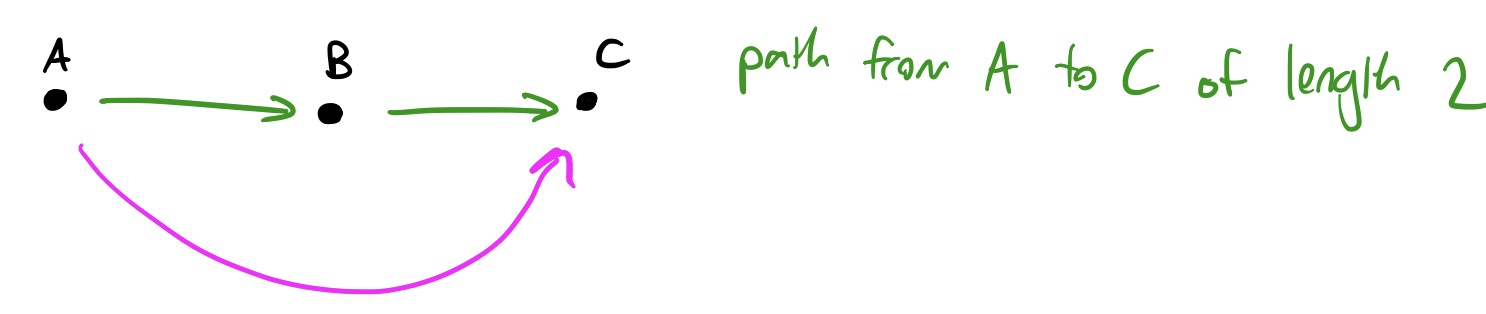
\includegraphics[width=1.2\linewidth]{graph/16.jpg} \\% 调整图片大小和图片路径
\\
There is a \hl{path of length k from x to y} in R if there are\\
$x = x_0,..., x_k = y$ such that $xRx_1, x_0Rx_1, ..., x_{k1}Ry.$
\begin{center}
There is a path of length k from x to y if and only if $xR^{k}y$.
\end{center}

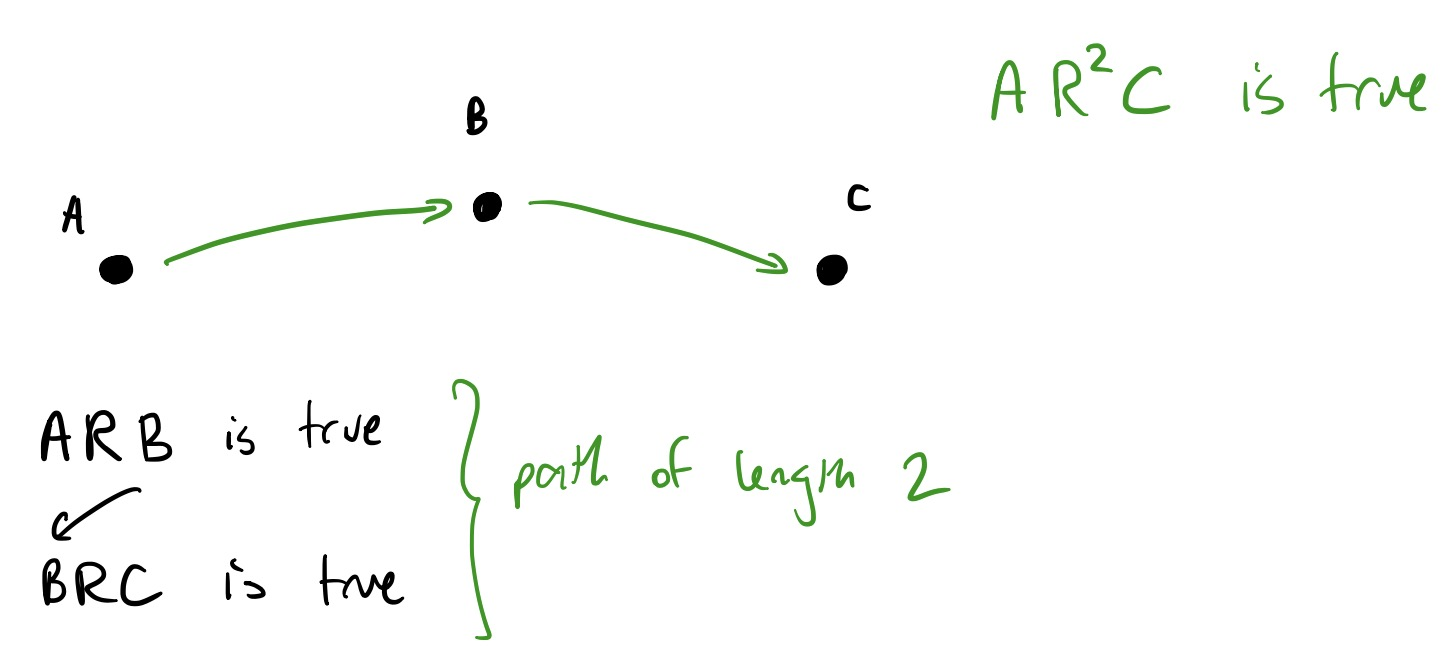
\includegraphics[width=0.8\linewidth]{graph/17.jpg} \\% 调整图片大小和图片路径
\\
connectivity closure:
\begin{center}
\hl{$R^* = \bigcup_{k=1}^{\infty}$}\\
or \\
$R \cup R^2 \cup R^3 \cup R^4 ......$
\end{center}


\textbf{\hl{Short summary}}
\begin{itemize}
\item The connectivity closure $R^*$ is the transitive closure tra(R).
\item If X has only n elements,  then $R^* = \bigcup^n_{k=1} R^k$
\end{itemize}

================================================================================================================
\newpage
================================================================================================================\\

\textbf{Example}\\
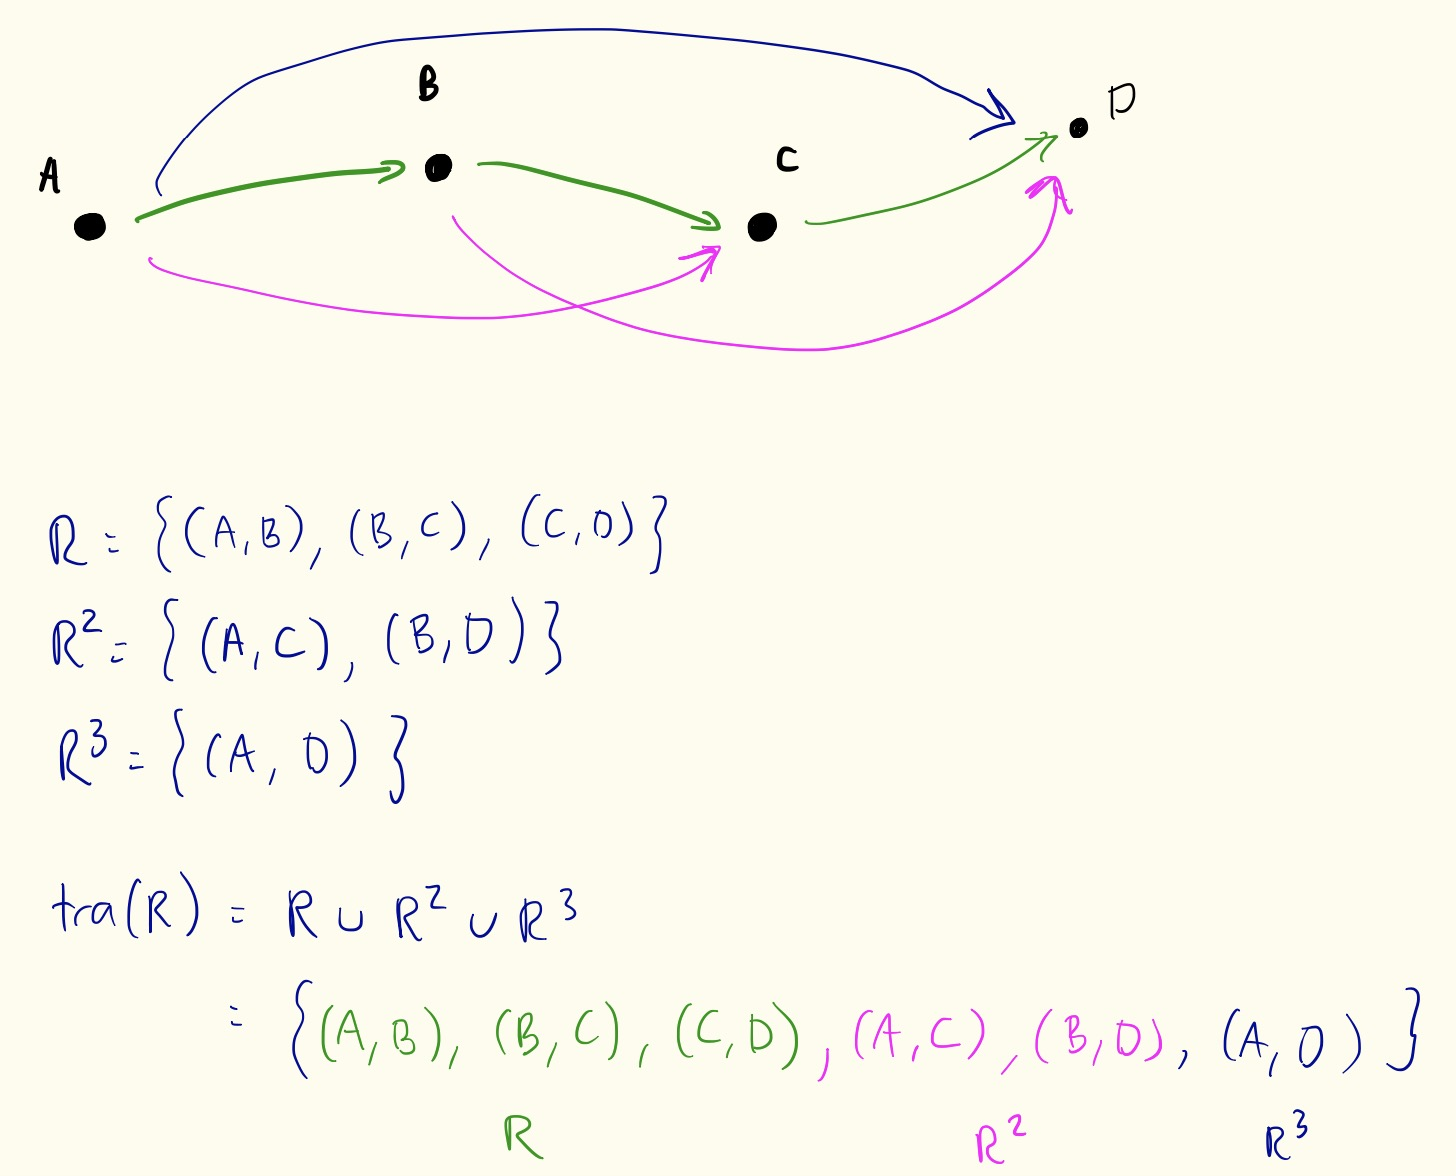
\includegraphics[width=0.8\linewidth]{graph/18.jpg} \\% 调整图片大小和图片路径

\item \hl{Warshall’s algorithm}
\hl{Main idea}: A path exists between vertices x and y if and only if:
\begin{itemize}
\item there is an edge from x to y; or
\item there is a path from x to y going through vertex 1; or
\item there is a path from x to y going through vertices 1 and/or 2; or
\item ...
\item there is a path from x to y going through any of the other n  2
vertices.
\end{itemize}

================================================================================================================
\newpage
================================================================================================================\\

\textbf{Example}
\begin{center}
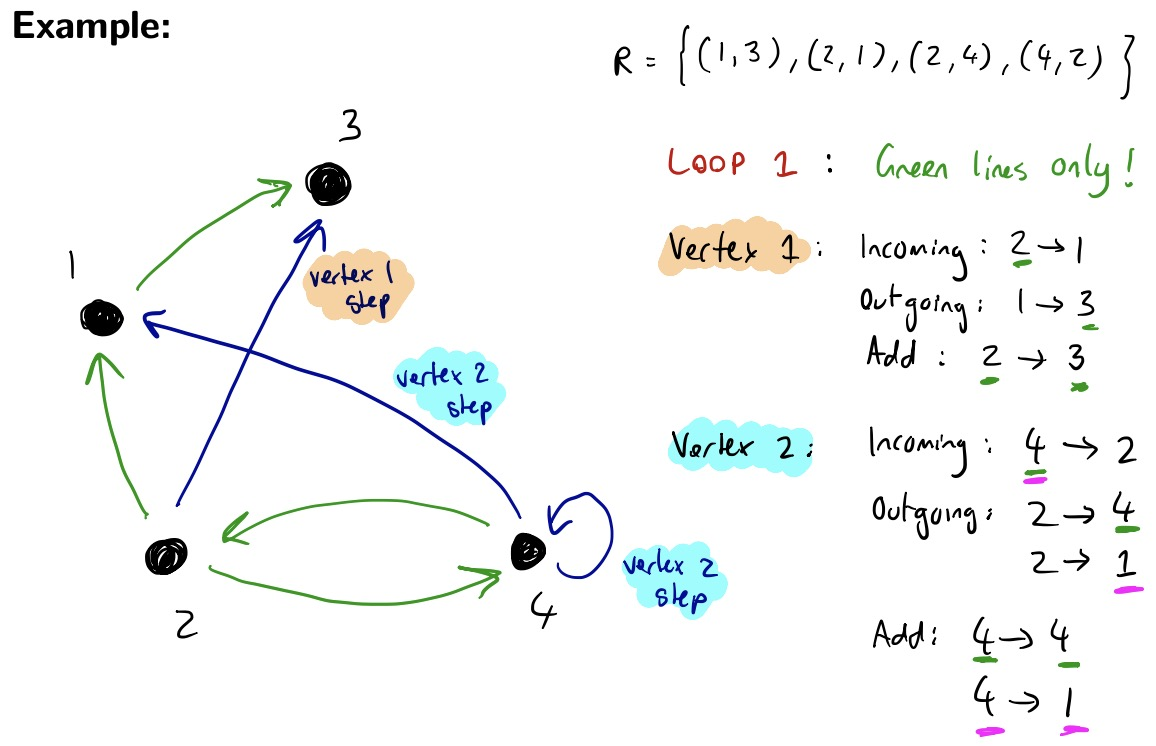
\includegraphics[width=0.6\linewidth]{graph/19.jpg} \\% 调整图片大小和图片路径
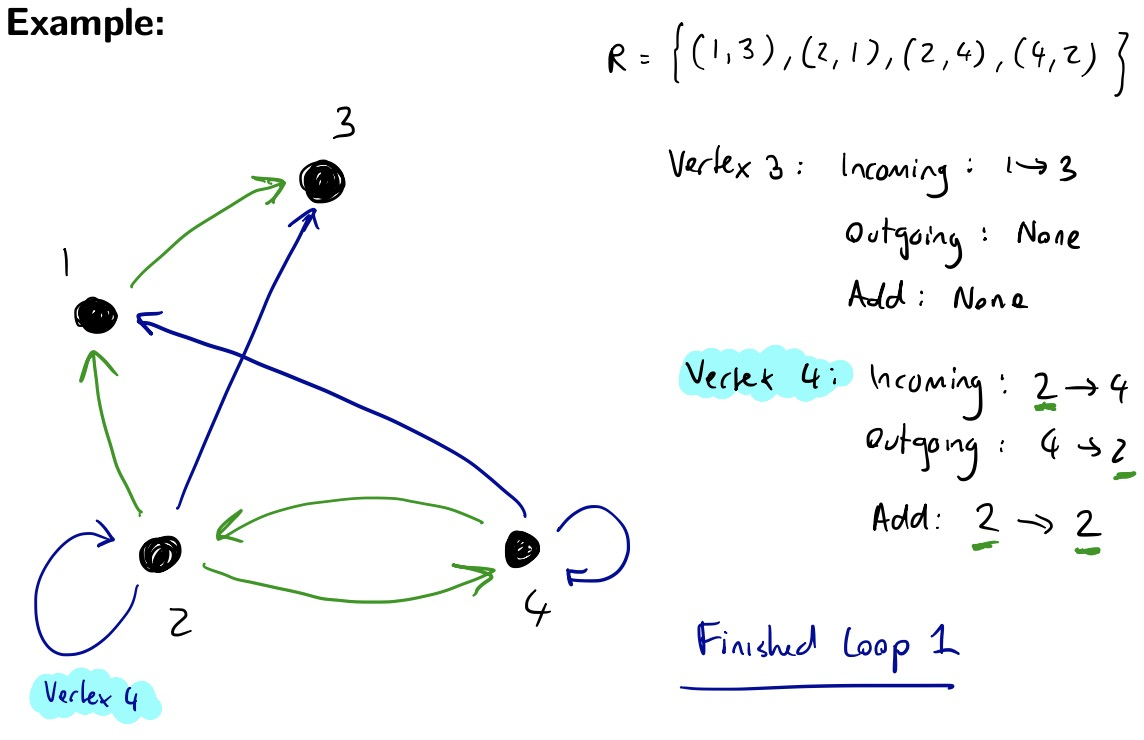
\includegraphics[width=0.6\linewidth]{graph/20.jpg} \\% 调整图片大小和图片路径
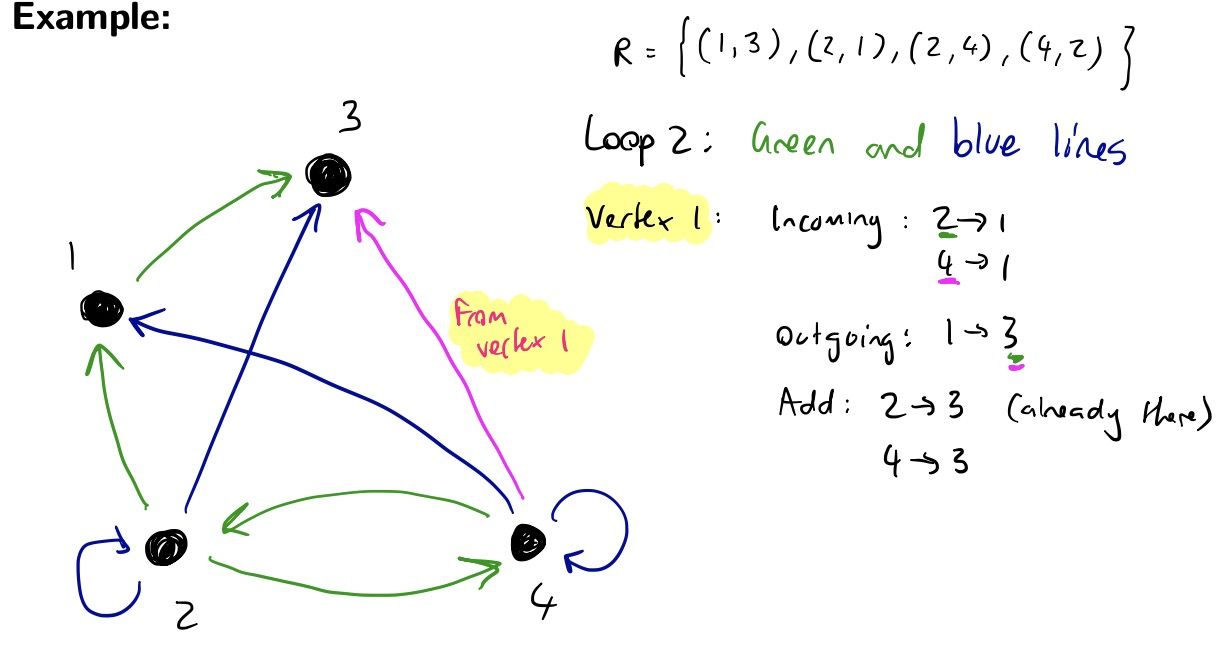
\includegraphics[width=0.6\linewidth]{graph/21.jpg} \\% 调整图片大小和图片路径
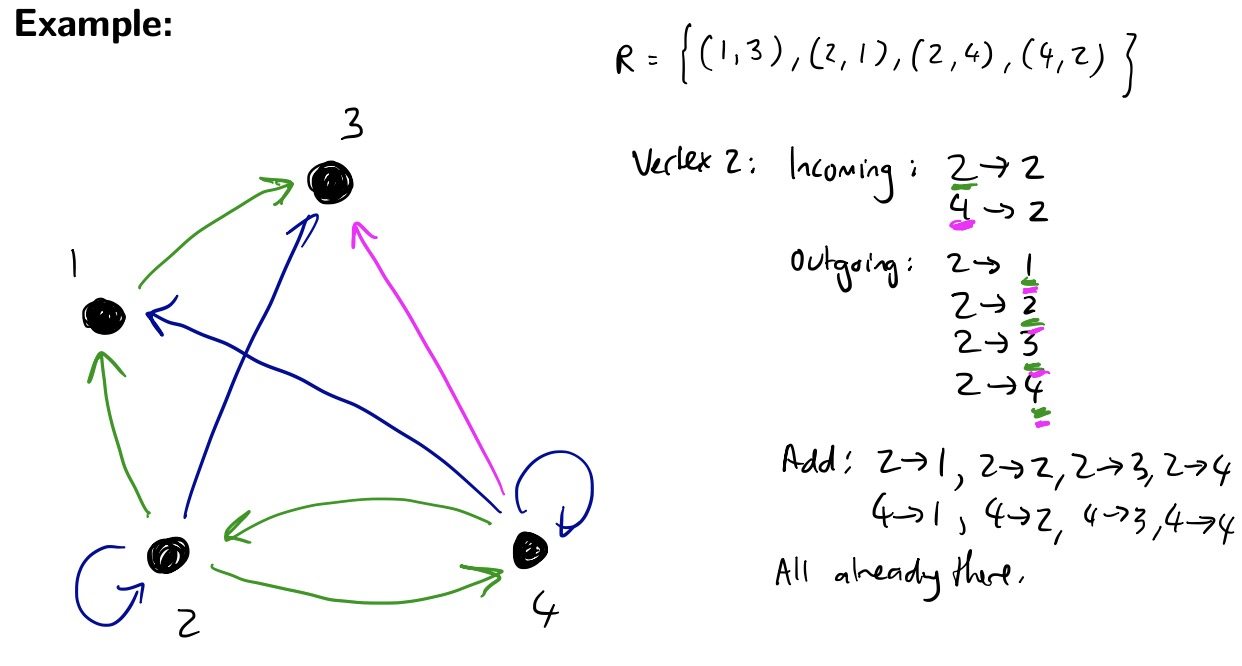
\includegraphics[width=0.6\linewidth]{graph/22.jpg} \\% 调整图片大小和图片路径
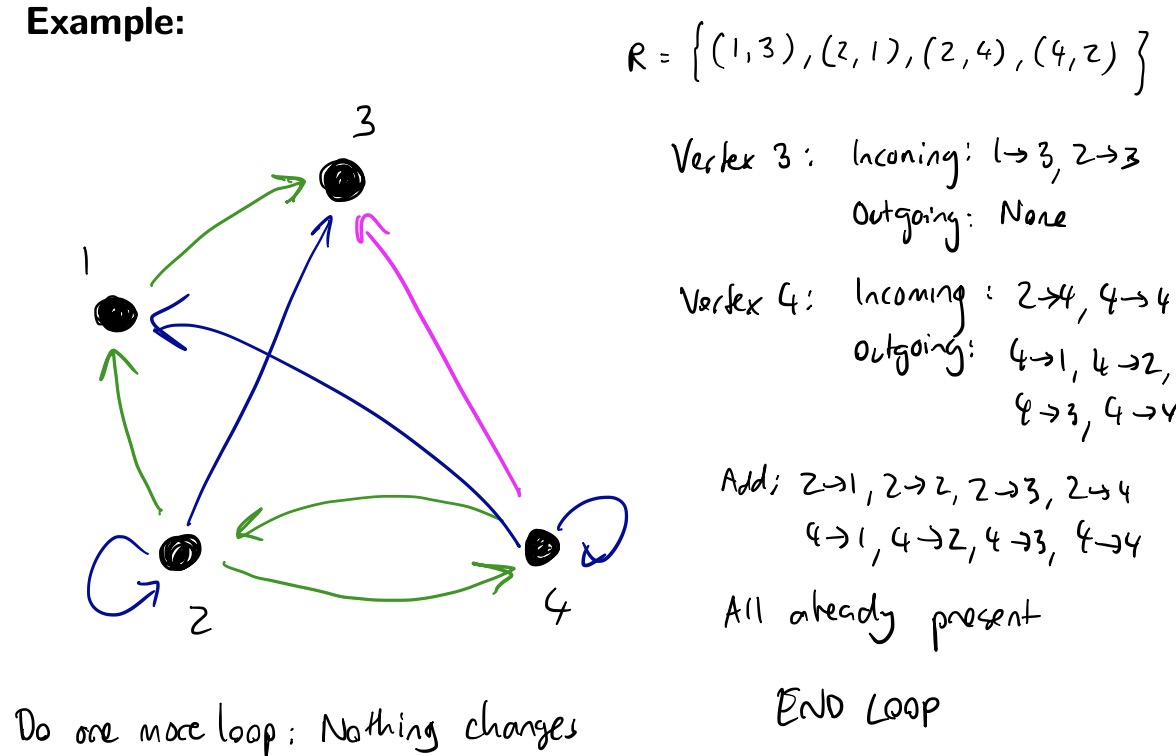
\includegraphics[width=0.6\linewidth]{graph/23.jpg} \\% 调整图片大小和图片路径
\end{center}


\item \hl{Order of taking closures}
\begin{itemize}
\item ref(sym(R)) = sym(ref(R))
\item ref(tra(R)) = tra(ref(R))
\item tra(sym(R)) = sym(tra(R))
\end{itemize}

================================================================================================================
\newpage
================================================================================================================\\

\section {W11} 

\item Graph theory\\
A \hl{graph} G consist of 2 \hl{finite} sets:
\begin{itemize}
\item a \hl{non-empty} set V(G) of vertices
\item a \hl{possibly empty} set E(G) of edges, where associated with a set $\{v,w\} \subseteq V(G)$\\
The vertices v and w are called the \hl{endpoints} of the edge.
\item A graph G is defined \hl{purely} in terms of sets V(G) and E(G).
The drawing is just a visual aid.
\item An edge may have endpoints {v, v}\\
We call such an edge a \hl{loop}
\item 2 edges may have the same endpoints $\{v,w\}$.
We call these \hl{parallel edges}.
\item A graph with \hl{no loops or parallel edges} is called a \hl{simple graph}.
\end{itemize}

\item Peterson Graph\\
most famous counter \hl{example}\\
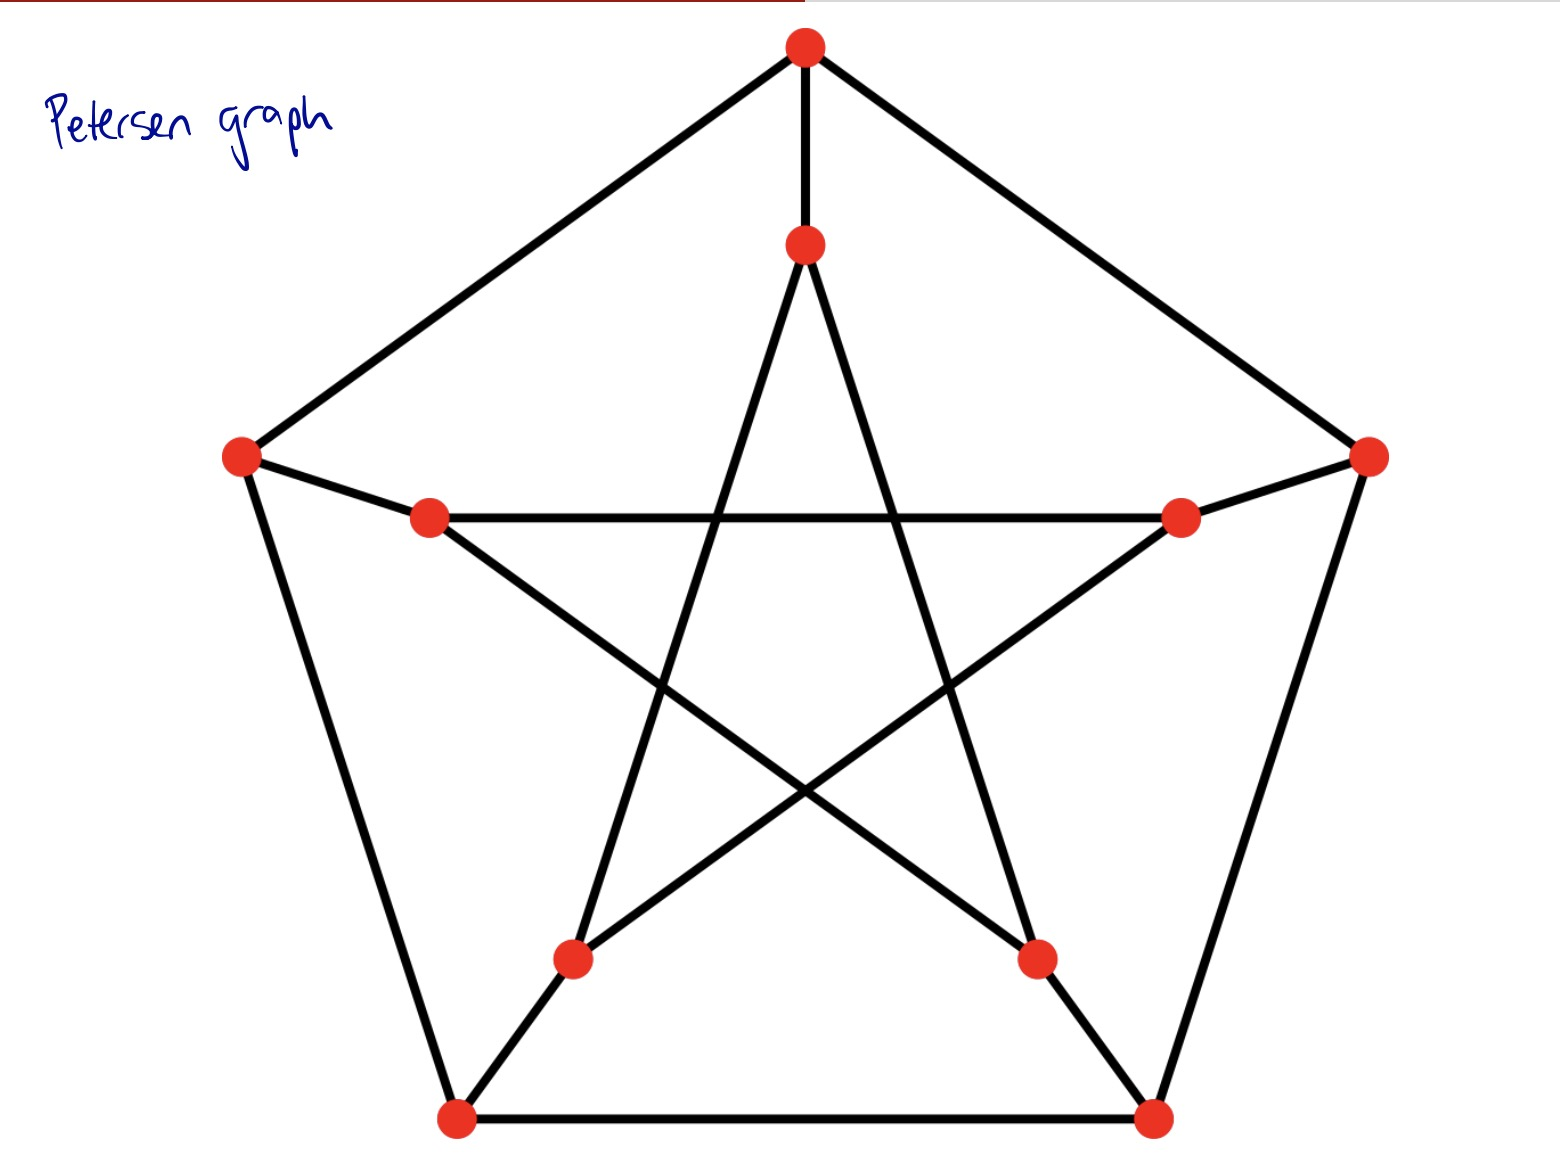
\includegraphics[width=0.6\linewidth]{graph/24.jpg} \\% 调整图片大小和图片路径


================================================================================================================
\newpage
================================================================================================================\\


\item Terminologies
\begin{itemize}
\item \textbf{Incident} : For an edge e and a vertex v ,  v is an endpoint of e
\item \textbf{adjacent} : For vertices $u,v$,  there is an edge with endpoints  $\{u,v\}$\\
A vertex u is adjacent to itself if there is a \hl{loop} with endpoints $\{u\}$.
\item \textbf{Degree}  : the degree of vertex v is the number of edges incident with v , where we count each \hl{loop twice} ,we write this as deg(v).\\
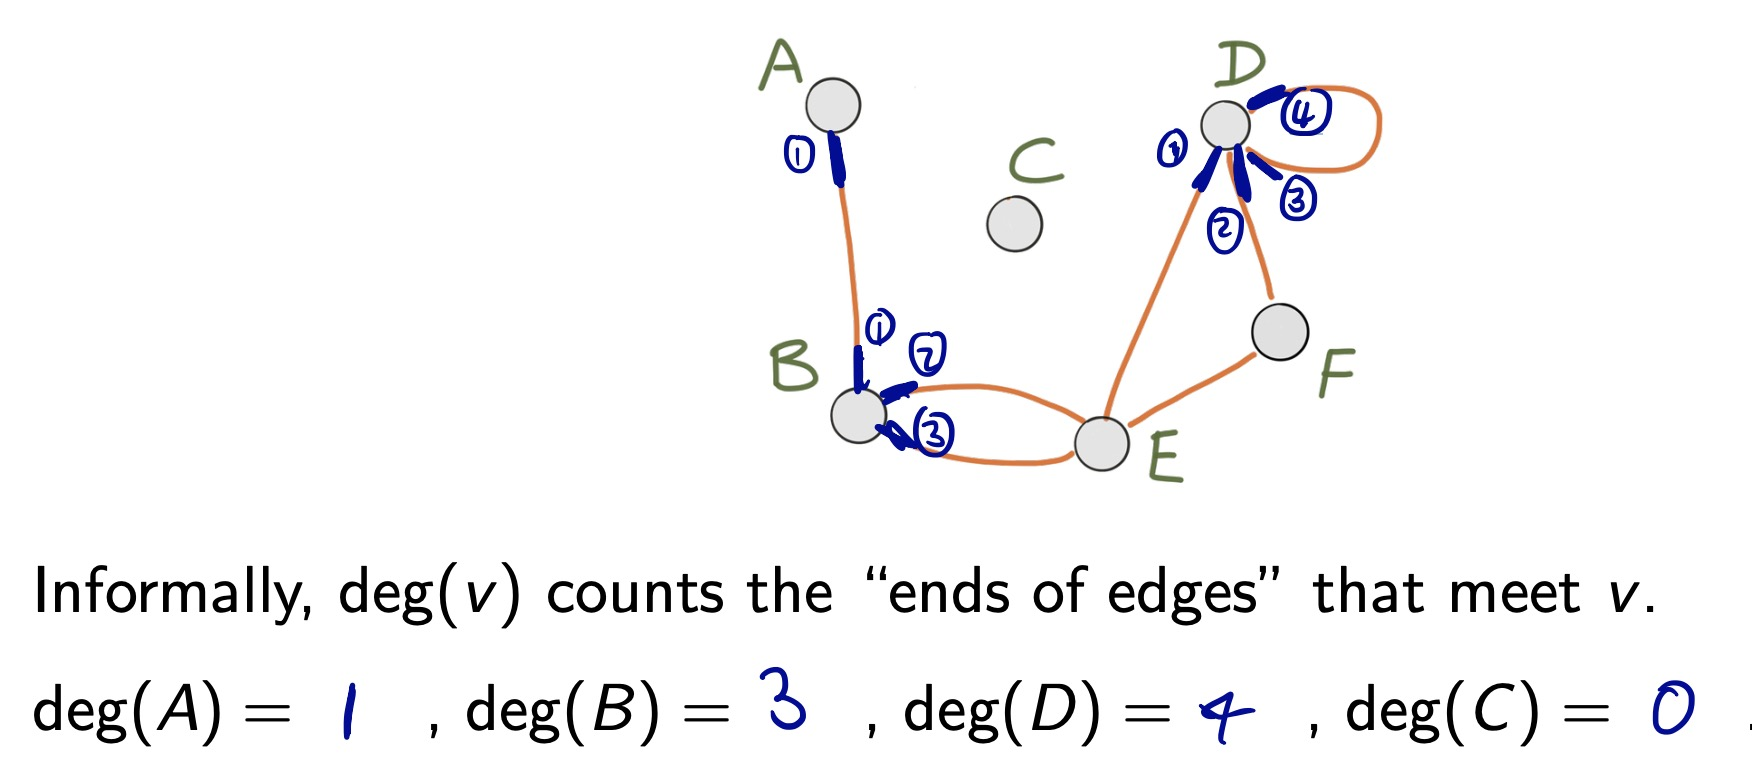
\includegraphics[width=1\linewidth]{graph/25.jpg} \\% 调整图片大小和图片路径
\end{itemize}

\item \textbf{Handshake Theorem}\\
Let G be a graph with n vertices $V(G) = \{v_1,v_2...v_n\}$,Then 
\begin{center}
$\sum_{i=1}^n deg(v_1)  = deg(v_1) + ......  + deg(v_n) = 2 \cdot |E(G)|$
\end{center}
In particular, in any graph, the sum of all vertex degrees must be even.


\item Directed graphs\\
Let G be a digraph (directed graph), and $v \in V(G)$
\begin{itemize}
\item The in-degree $def^{-} (v)$ is the number of edges \hl{terminating} in v.
\item The out-degree $deg^{+} (v)$ is the number of edges \hl{starting} in v. 
\end{itemize}

Let G be a directed graph with n vertices $ V(G) = \{v_1,..., v_n\} $ Then:
\begin{center}
$\sum^{n}_{i = 1} deg^{-} (vi) = \sum^{n}_{i = 1} deg^{-} (vi) = |E(G)|$
\end{center}

\item \hl{Path}\\
Let G be a graph and let $x,y \in V(G)$ . A \hl{path} in G from x to y is an alternating sequence of vertices and edges:
\begin{center}
$v_0$(starting vertex)$,e_1,v_1,e_2,...,v_{n-1},e_n,v_n$(end vertex)
\end{center}
where $v_0 = x, v_n = y$, and each edge $e_i$ has endpoints $\{v_{i-1} , v_i\}$\\
================================================================================================================
\newpage
================================================================================================================\\


\item More on path
\begin{itemize}
\item \hl{Connected graph and Disconnected} : for a graph G, $\forall$ vertices $x,y \in V(G)$, there is a path from x to y. Otherwise G is called disconnected.

\end{itemize}

\item \hl{Circuit}\\
A path is called a \hl{circuit} if it \hl{does not repeat any edge},
and it starts and ends at the \hl{same vertices}.

\item \textbf{Eulerian circuits}\\
A Eulerian circuit is a \hl{path} that starts and ends at the \hl{same vertex}, and
that uses \hl{every edge exactly once}.
\begin{itemize}
\item If we ignore isolated vertices(degree = 0), the the remaining graph must be connected.
\item Let G be a connected graph. Then G has a Eulerian circuit \hl{if and only if} every vertex of G has \hl{even degree} .
\end{itemize}

\item \textbf{Eulerian trail} \\
A \hl{Eulerian trail} is a \hl{path} using \hl{each edge exactly} once, but whose start
and end vertices \hl{can be different}.

\begin{center}
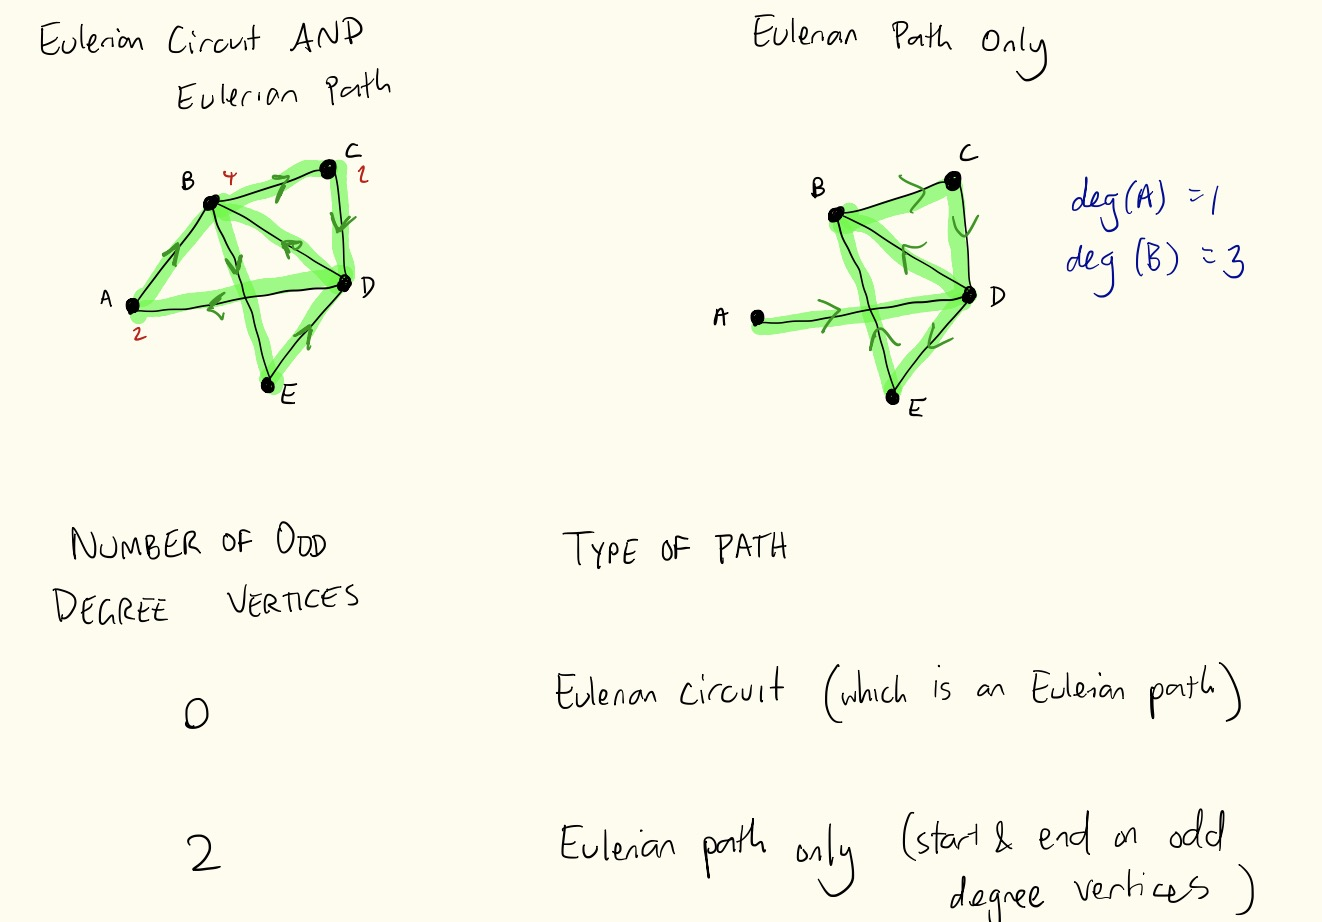
\includegraphics[width=1\linewidth]{graph/28.jpg} \\% 调整图片大小和图片路径\\
\end{center}


\item Hamiltonian circuits\\
circuit using every \hl{vertex
exactly once}. (Except for start = end vertex, which must appear twice.)

\item \hl{Graph isomorphism}\\
Two graphs $G_1 = (V_1,E_1)$ and $G_2 = (V_2,E_2)$ are said to be \hl{isomorphic} written $G_1 \cong G_2$,  if there exists a bijective function $f: V_1 \rightarrow V_2$ such that:
\begin{center}
$f(E_1) = \{\{f(v_1),f(v_2)\} | \{v_1,v_2\} \in E_1\} = E_2$ 
\end{center}

\begin{center}
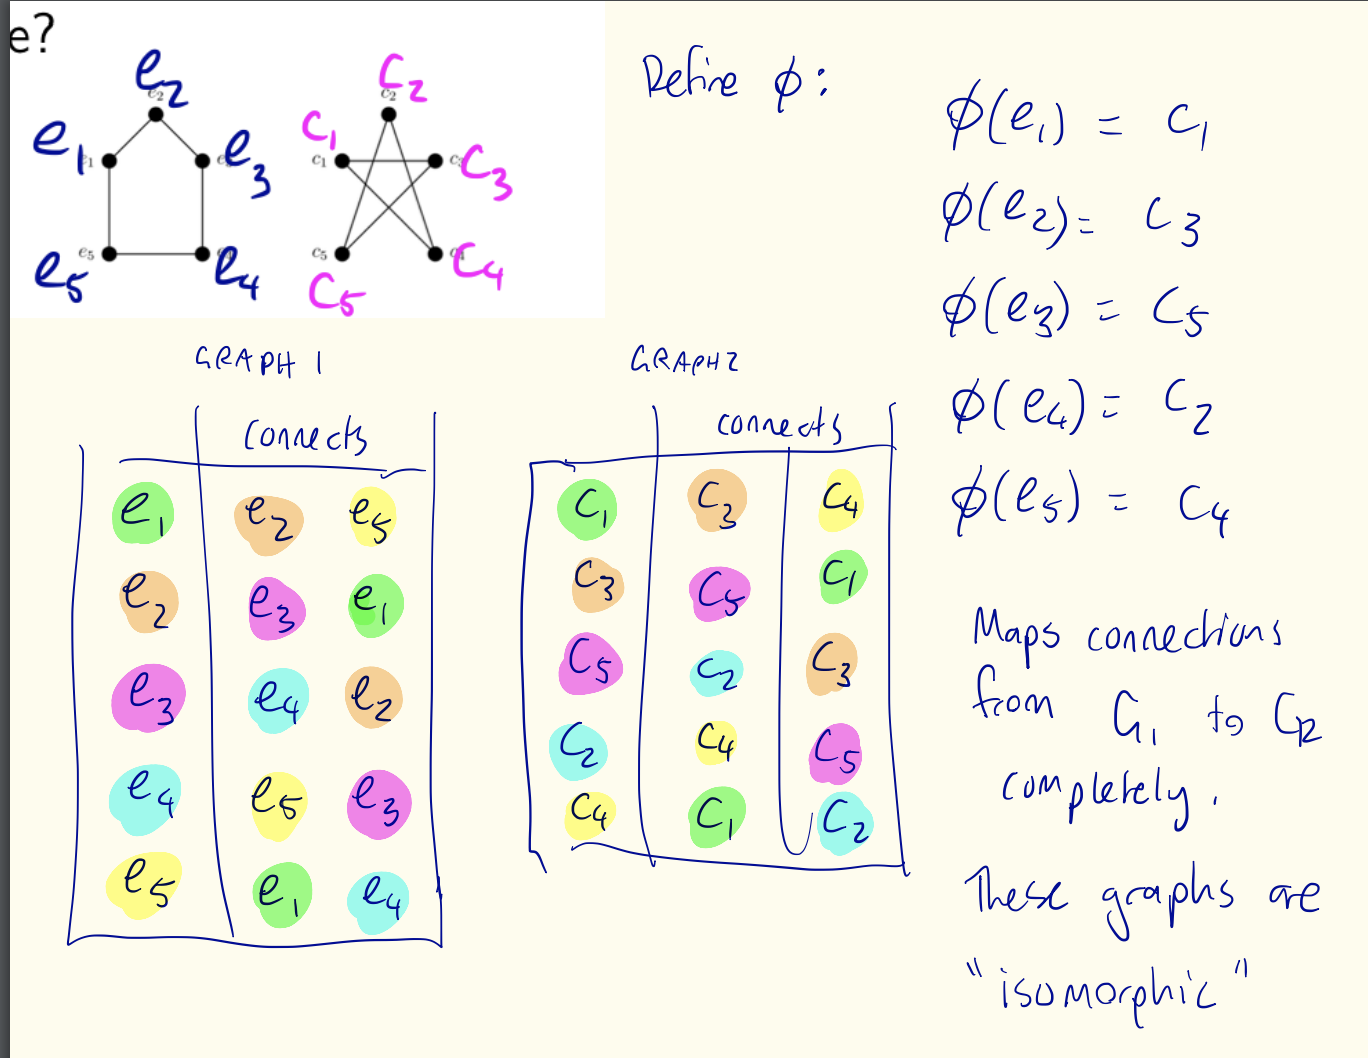
\includegraphics[width=0.6\linewidth]{graph/26.jpg} \\% 调整图片大小和图片路径
\end{center}

\item \textbf{Representing graphs using Matrices}\\
Let G a graph with n vertices, and suppose we label these vertices
$V(G) = \{1, 2,..., n\}$\\
The adjacency matrix of $G$ is the $n \cdot n$ matrix $\mathbb{A} =(a_{i,j})$, where each entry $a_{i,j}$ is the \hl{number of edges} with endpoints $\{i,j\}$\hl{(counted with multiplicity)}\\
\begin{center}
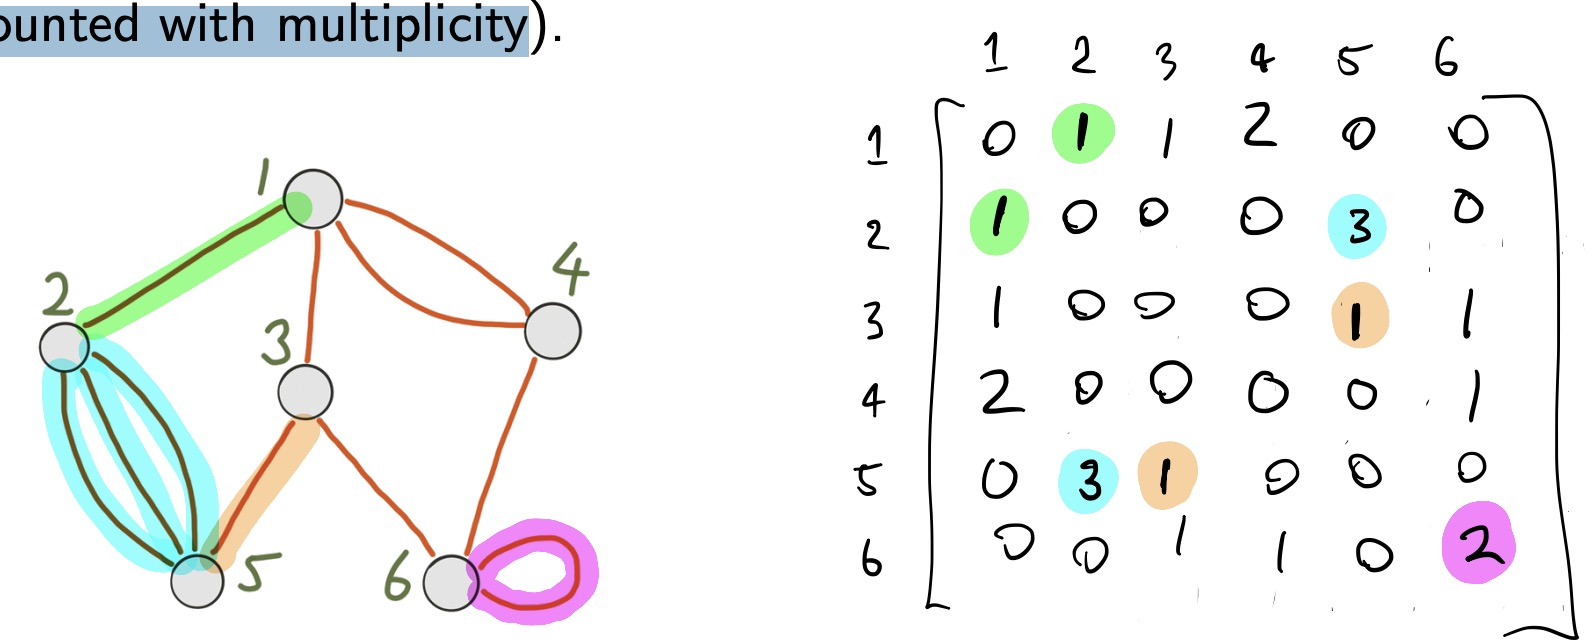
\includegraphics[width=0.8\linewidth]{graph/27.jpg} \\% 调整图片大小和图片路径
\end{center}
\hl{\textbf{Theorem}}


Let G be a graph with vertices $V(G) = \{1, 2,..., n\}$, and
\textbf{adjacency matrix} $\mathbb{A}$.\\
Then the \hl{number of paths of length k} from vertex i to vertex j is the
entry in row i, column j of the kth power $A_k = A \cdot A \cdot ...  A$.

================================================================================================================
\newpage
================================================================================================================\\

\section{W12}

\item \textbf{Bipartite graph}\\
The simple graph G is \hl{bipartite} if it has \hl{at least 2 vertices} and satisfies
one (and hence all) of the following equivalent conditions:
\begin{itemize}
\item The set of vertices $V(G)$ has a partition $\{V_1,V_2\}$ such that every edge is of the form $\{v_1,v_2\}$ where $v_k \in V_k$
\begin{center}
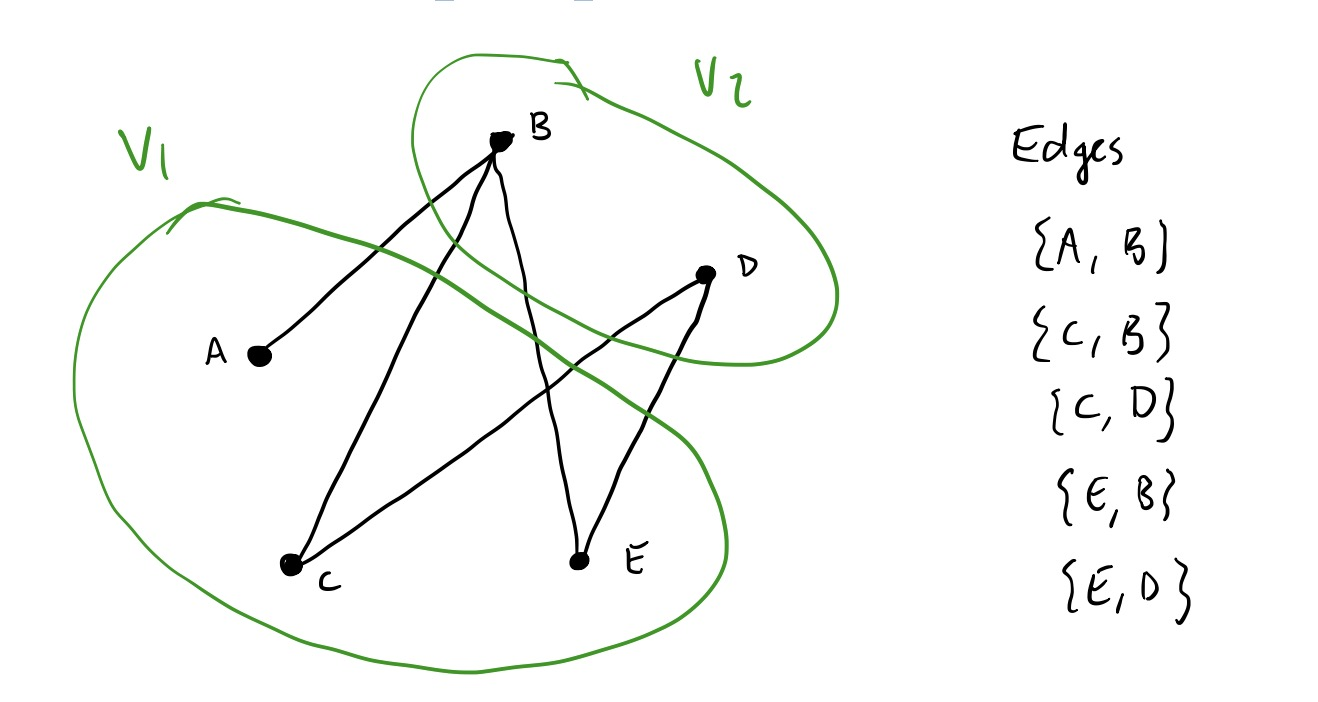
\includegraphics[width=0.8\linewidth]{graph/29.jpg} \\% 调整图片大小和图片路径
\end{center}

\item The vertices can be coloured with two colours such that \hl{no two
adjacent vertices} have the same colour\\
\begin{center}
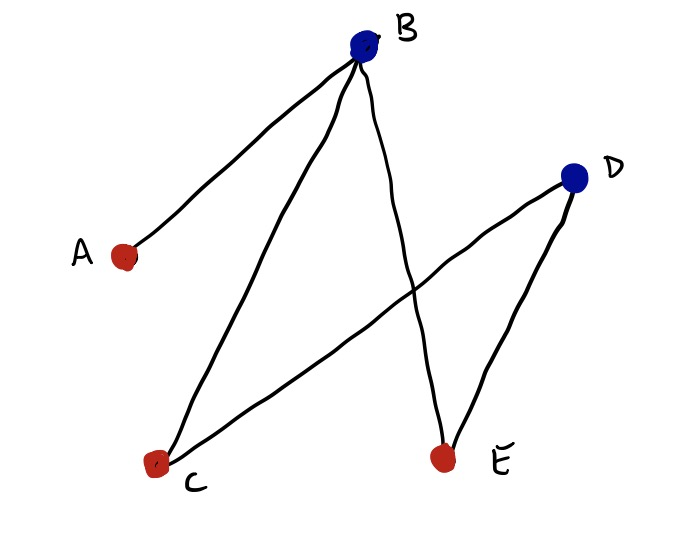
\includegraphics[width=0.7\linewidth]{graph/30.jpg} \\% 调整图片大小和图片路径
\end{center}

================================================================================================================
\newpage
================================================================================================================\\
\item Every circuit in G has even length.
\begin{center}
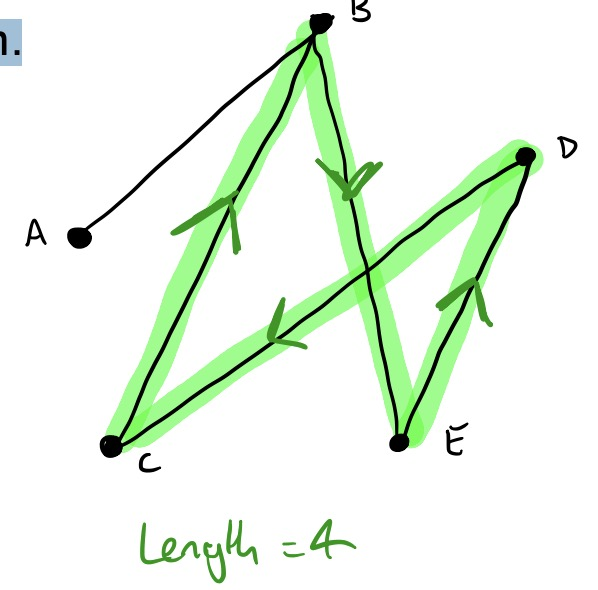
\includegraphics[width=0.7\linewidth]{graph/31.jpg} \\% 调整图片大小和图片路径
\end{center}
\end{itemize}

================================================================================================================
\newpage
================================================================================================================\\

\item \textbf{Finite state machine (with output)}\\
A finite state machine (with output) M = (S, I, O, f , g,s0) consists of
\begin{itemize}
\item a finite set \hl{S} of states
\item a finite input alphabet \hl{I}
\item a finite output alphabet \hl{O}
\item  transition function $f : S \times I \rightarrow S$
\item an output function $g : S \times I \rightarrow O$
\item an initial state $s_0$
\end{itemize}

\item Representing finite state machines: State diagrams\\
A more visual representation of a finite state machine
$M = (S, I, O, f , g,s0)$, is via a digraph, with one vertex per state and one
directed edge per transition, each decorated with input and output.\\
\textbf{Example}
\begin{itemize}
\item $S = \{s_0,s_1,s_2,s_3,s_4,s_5,s_6\}$
\item $I = \{5,10,25,O,R\}$
\item $O = \{n,5,10,25,orange juice,apple juice\}$
\item f
\item g
\item $s_0$
\end{itemize}


\item Formal languages\\
Let \textbf{A} be a finite set called the alphabet.\\
A \hl{formal language} \textbf{L} is set of strings with symbol in \textbf{A}.\\
The empty string is denoted $\lambda$.\\
\textbf{Example}
\begin{itemize}
\item $A = \{0,1\}, L = \{0^{n}1^m | m,n in \mathbb{N}\}$
\item $A = \{0,1\}, L = \{0^{n}1^n |  n in \mathbb{N}\}$
\item $A = \{a,b,c,d,.....,z\}, $L = all English words
\end{itemize}


================================================================================================================
\newpage
================================================================================================================\\

\item \textbf{Phrase-structure grammar}\\
A phrase-structure grammar $G = (V,T, S, P)$ consists of
\begin{itemize}
\item a vocabulary (or alphabet) V
\item a subset $T \subseteq V$ of terminal symbols
\item a start symbol $S \in V $
\item a finite set of productions P\\
The non-terminal symbols are N = V - T. Every production in P must
have at least one non-terminal symbol on its \hl{left side}.
\end{itemize}
The \hl{language generated by G} is the set \hl{L(G)} of all words in terminals that
can be derived from S using the productions P.\\
The set of all sentences (or words) over V is $V^*$.
So \hl{$L(G) \subseteq T^* \subseteq V^*$}.\\\\
\textbf{Example}\\
G = (V,T, S, P) where\\
V = {0, 1, S, A} (vocabulary or alphabet),\\
T = {0, 1} (terminal symbols),\\
P = {$S \rightarrow 0A, S \rightarrow 0S, A \rightarrow 1A, A \rightarrow 1$} (productions)\\
\textbf{So that}\\
\hl{$V^*$} is the set of all words in V, e.g 01AAA1,SSA101, $\lambda$(empty string)\\
\hl{$T^*$} is the set of all words i T. e.g. 001,101,$\lambda$\\
\hl{$L(G) \subseteq T^* \subseteq V^*$}.


================================================================================================================
\newpage
================================================================================================================\\


\item \textbf{Types of grammars: The Chomsky Hierarchy}\\

\begin{center}
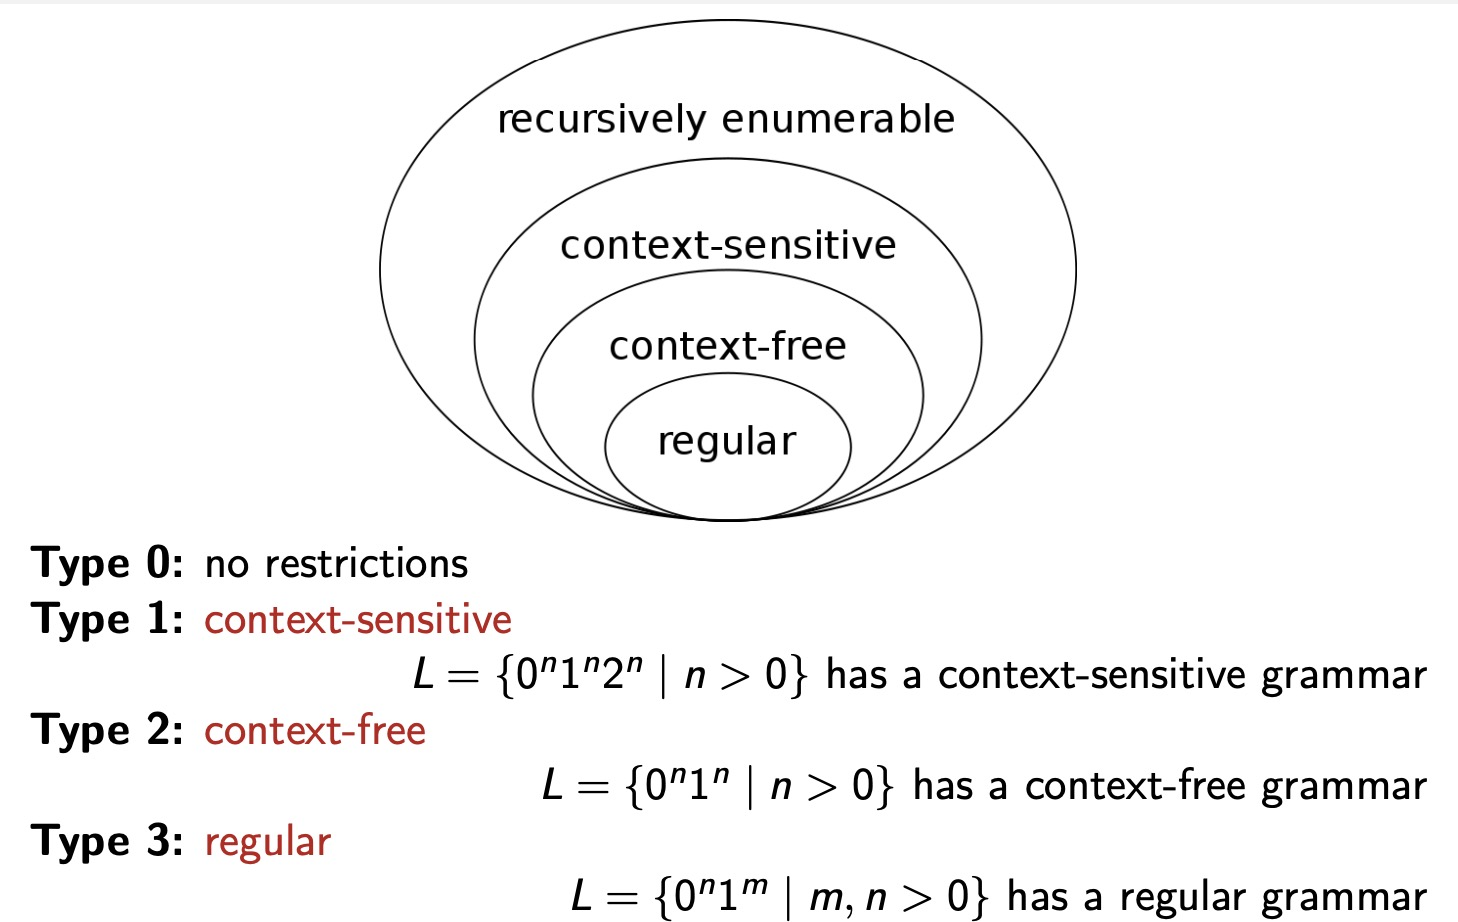
\includegraphics[width=0.6\linewidth]{graph/32.jpg} \\% 调整图片大小和图片路径
\end{center}

\begin{center}
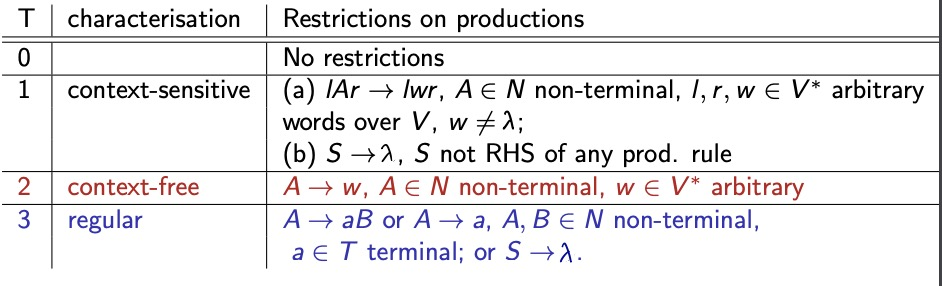
\includegraphics[width=0.86\linewidth]{graph/33.jpg} \\% 调整图片大小和图片路径
\end{center}

================================================================================================================
\newpage
================================================================================================================\\
\section{W13}

\item *
\begin{center}
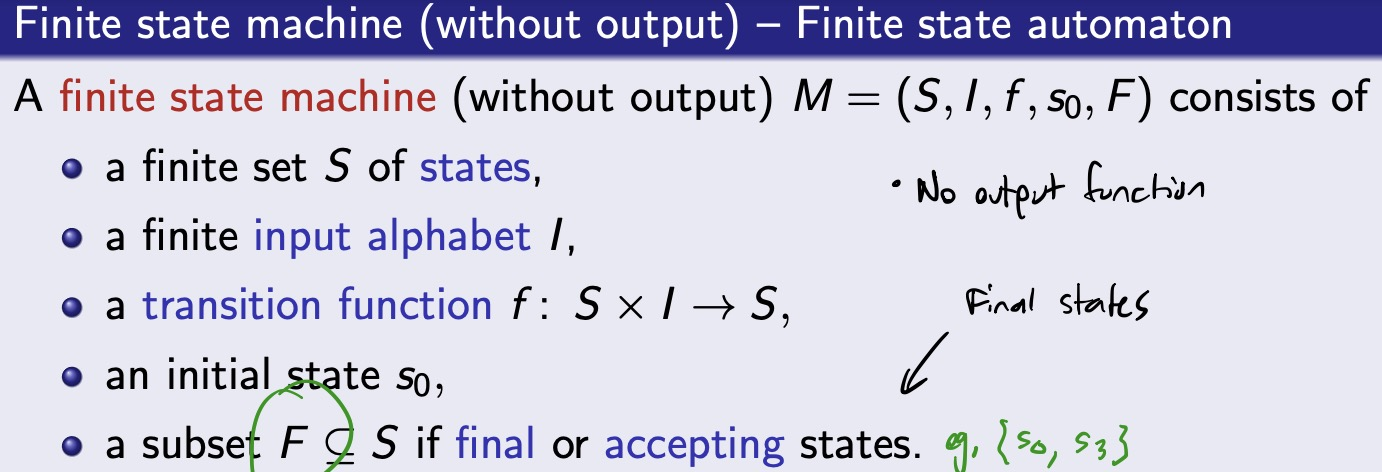
\includegraphics[width=0.86\linewidth]{graph/36.jpg} \\% 调整图片大小和图片路径
\end{center}

\item Extended transition function and Recognised language\\
\begin{center}
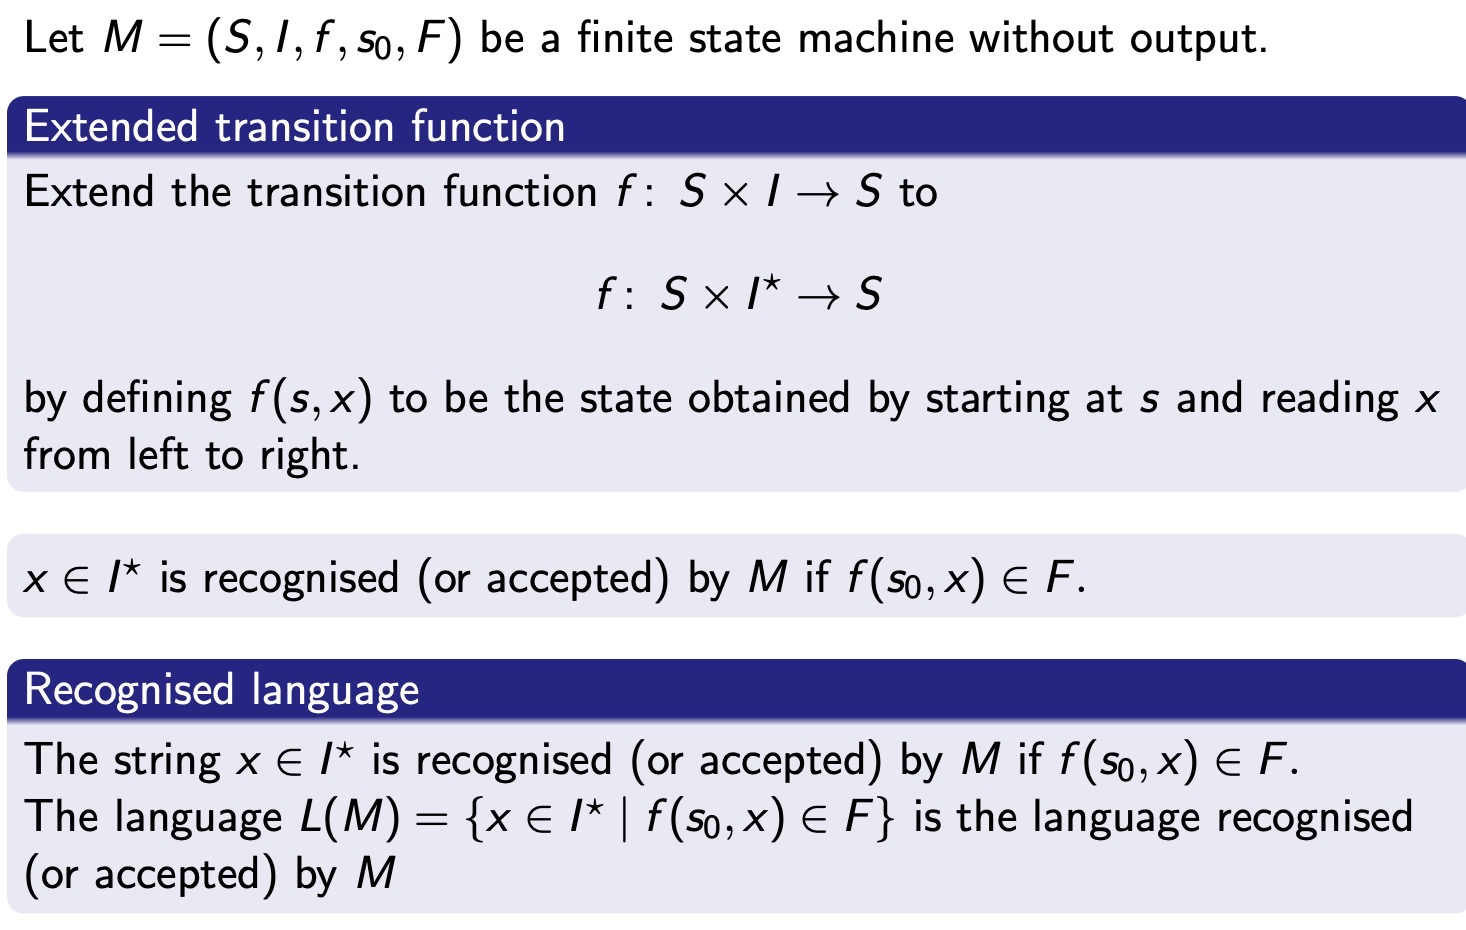
\includegraphics[width=0.86\linewidth]{graph/35.jpg} \\% 调整图片大小和图片路径
\end{center}

\end{itemize} %1

\end{document}

